%# -*- coding: utf-8-unix -*-
%%==================================================
%% thesis.tex
%%==================================================

% 双面打印
%\documentclass[doctor, fontset=adobe, openright, twoside]{sjtuthesis}
% \documentclass[bachelor, fontset=adobe, openany, oneside, submit]{sjtuthesis} 
\documentclass[master, adobefonts, zihao=-4]{sjtuthesis} 
% \documentclass[%
%   bachelor|master|doctor,	% 必选项
%   fontset=adobe|windows,  	% 只测试了adobe
%   oneside|twoside,		% 单面打印,双面打印(奇偶页交换页边距,默认)
%   openany|openright, 		% 可以在奇数或者偶数页开新章|只在奇数页开新章(默认)
%   zihao=-4|5,, 		% 正文字号:小四、五号(默认)
%   review,	 		% 盲审论文,隐去作者姓名、学号、导师姓名、致谢、发表论文和参与的项目
%   submit			% 定稿提交的论文,插入签名扫描版的原创性声明、授权声明 
% ]

% 逐个导入参考文献数据库
\addbibresource{bib/thesis.bib}
% \addbibresource{bib/chap2.bib}
\usepackage{pifont}
\usepackage{url}
\usepackage{tabularx}
\newcommand{\xmark}{\ding{55}}
\newcommand{\cmark}{\ding{51}}
\renewcommand{\texttt}[1]{%
  \begingroup
  \ttfamily
  \begingroup\lccode`~=`/\lowercase{\endgroup\def~}{/\discretionary{}{}{}}%
  \begingroup\lccode`~=`[\lowercase{\endgroup\def~}{[\discretionary{}{}{}}%
  \begingroup\lccode`~=`.\lowercase{\endgroup\def~}{.\discretionary{}{}{}}%
  \catcode`/=\active\catcode`[=\active\catcode`.=\active
  \scantokens{#1\noexpand}%
  \endgroup
}
\begin{document}

%% 无编号内容:中英文论文封面、授权页
%# -*- coding: utf-8-unix -*-
\title{ANDROID应用审核系统的设计与实现}
\author{袁\quad{}理}
\advisor{戚正伟}
% \coadvisor{某某教授}
\defenddate{2017年1月10日}
\school{上海交通大学}
\institute{电子信息于电气工程学院}
\studentnumber{1140379051}
\major{软件工程}

\englishtitle{Design and Implementation of an Android Application Auditing System}
\englishauthor{\textsc{Li Yuan}}
\englishadvisor{Prof. \textsc{ZhengWei Qi}}
% \englishcoadvisor{Prof. \textsc{Uom Uom}}
\englishschool{Shanghai Jiao Tong University}
\englishinstitute{\textsc{School of Electronics, Information and Electrical Engineering} \\
  \textsc{Shanghai Jiao Tong University} \\
  \textsc{Shanghai, P.R.China}}
\englishmajor{Software Engineering}
\englishdate{Jan, 2017}


\maketitle

\makeenglishtitle

\makeatletter
\ifsjtu@submit\relax
	\includepdf{pdf/original.pdf}
	\cleardoublepage
	\includepdf{pdf/authorization.pdf}
	\cleardoublepage
\else
	\makeDeclareOriginal
	\makeDeclareAuthorization
\fi
\makeatother


\frontmatter 	% 使用罗马数字对前言编号

%% 摘要
\pagestyle{main}
%# -*- coding: utf-8-unix -*-
%%==================================================
%% abstract.tex for SJTU Master Thesis
%%==================================================

\begin{abstract}
如今,各种各样的手机应用正在丰富人们的生活。应用市场作为应用发布与分发的入口,已经在移动生态中扮演了至关重要的角色。
Android秉承的“开放”的观念造就了Android生态圈的繁荣,但同时也使得应用市场变得碎片化。
而在移动应用使得人们生活更简单更舒适的同时,很多具有恶意行为和病毒的应用也悄悄侵蚀着人们的手机。
这些应用可能会导致用户的隐私数据泄露,财产遭到损失。
频发的移动安全事件说明了目前应用市场的确存在审核不严的情况。


目前威胁用户手机安全的应用可以大致分为以下三类:1. 盗取用户隐私信息的恶意应用;2. 克隆应用;3. 使用了存在隐私泄露问题或安全漏洞的第三方库的应用。
针对以上三个问题,本文设计了一个应用审核系统AppShield。
AppShield整合了AppAudit,对单应用进行审查。
同时我们基于AppAudit的检测结果,进一步分析,通过文件特征和包标识符识别问题组件,并在测试集中检测问题部件的不同版本,总结报告。
另外,我们提出了一种相似度检测方法,能在应用被混淆的情况下,检测应用之间的相似度。
通过对混淆技术的学习,我们总结出了一组稳定特性,即在混淆前后基本上不会改变的特性。
基于稳定特性,我们能对应用进行指纹提取,并进行比对,从而对计算出应用之间的相似度。
该方法被应用于AppShield系统中,对应用进行克隆应用以及第三方库的检测。


为了测试AppShield的审核效果,我们经过两年时间,收集了将近14万个来自国内外不同应用市场的应用,并将这些应用功能当做AppShield的测试集。
我们在近14万的应用上进行了隐私泄露检测,检测出了超过9000多例的隐私泄露应用,并总结出超过20个有隐私问题的问题部件。
同时我们挑选了8个第三方库的67个SDK版本,对来自腾讯应用宝市场的一万多个应用进行了第三方库检测。
检测结果表明,我们的检测方法检测出16.4\%的应用至少使用了一个我们挑选的第三方库。
其中Google处理JSON的工具库gson检测出占比最高,为10.26\%。
另外,我们随机挑选了1000个应用进行克隆应用检测,最终发现了一例开发者将应用以不同应用名多次提交至应用市场的案例。
测试与评估表明AppShield能够高效、准确的检测应用的隐私泄露问题,并找到存在问题的部件,同时有能力对应用进行相似度分析,从而找到存在问题的第三方库以及潜在的克隆应用。



\keywords{\large 隐私泄露 \quad 克隆应用 \quad 第三方库检测 \quad 相似度检测}
\end{abstract}

\begin{englishabstract}

Nowadays, smartphone plays a more and more important role.
Different mobile applications(or apps) make people's daily life colorful. 
Once an app releases, it will be distributed to an application store.
Then application store will deploy the app to the user's smartphone.
Thus it can be seen that application store plays a vital role in the mobile ecosystem.
While apps have made people's life simple, there are many apps which behave maliciously being installed to the user's device.
These apps may lead user's sensitive information leakage, make people's properties suffer great loss.
Frequently happened mobile security incidents indicate that the current application store lack of auditing.

There are three kinds of apps which will threaten the information security of mobile users: 1. Malware which will stole sensitive information; 2. clone app; 3. applications which use compromised third-party libraries.
To solve these problems, we propose AppShield, an Android application auditing system.
AppShiled integrates AppAudit which can identify the app which leaks user's sensitive information through hybrid program analysis.
AppShield concludes problematic components based on the analysis results of AppAudit and AppShield will study these components later.
We also propose a program analysis approach which can detect the similar packages, classes, and methods between apps even in the case of obfuscation.
AppShield uses this approach to detect third-party libraries and clone apps.

We have collected almost 140 thousands apps as the testset of AppShield through two years.
These apps are from different regions and different application stores.
We performed sensitive leakage detection through these apps, and detected more than 9,000 positive apps, and concluded more than 20 problematic components which will leak user's sensitive information.
We also performed third-party library detection through more than 10 thousands apps from myapp, one of the bigest application store in China.
We selected 8 distinct third-party libraries with 67 versions.
The analysis result shows that there are 16.4\% apps using at least 1 library we selected.
And Google's JSON utility library gson has the most popluate apps, 10.26\% in myapp.
In addition, we randomly selected 1,000 apps to perform our clone app detection. And we found that a developer distributed a same app with different app names twice to myapp.
The evaluation shows that AppShield can identify the app which leak sensitive information efficiently and accuratly.
And conclude the problematic components which have the same behaviors.
Also, AppShield has the ability to perform similarity analysis to apps to detect the victims of compromised third-party libraryies and clone apps.


\englishkeywords{\large Privacy leakage, clone application, third-library detection, similarity detection}
\end{englishabstract}



%% 目录、插图目录、表格目录
\tableofcontents
\listoffigures
\addcontentsline{toc}{chapter}{\listfigurename} %将插图目录加入全文目录
\listoftables
\addcontentsline{toc}{chapter}{\listtablename}  %将表格目录加入全文目录

\mainmatter	% 使用阿拉伯数字对正文编号

%% 正文内容
\pagestyle{main}
\chapter{绪论}
\label{chap:intro}

移动互联网随着智能手机的普及爆发,在智能手机上使用应用成为了日常生活中必不可少的部分,应用几乎涵盖了日常生活的所有部分,衣食住行等等都能通过应用来解决。
正是因为人们对应用的依赖如此之深,应用的安全性成为了各大应用市场需要解决的头号问题。
本章将首先在~\ref{sec:market-overview}节中介绍移动应用市场,然后~\ref{sec:market-prob}节会对应用市场面临的问题进行阐述与分析,最后在~\ref{sec:intro-conclusion}节中,本文将给出的解决方案进行一个大致的描述。

\section{移动应用市场现状}
\label{sec:market-overview}
截止到2016年第三季度, Android系统在全球移动操作系统市场份额中占86.8\%,IOS系统占12.5\%,这两大主流移动操作系统总共占比99.3\%,可以认为是整个市场的全部\footnote{Smartphone OS Market Share, 2016 Q3: \url{http://www.idc.com/prodserv/smartphone-os-market-share.jsp}}。
在腾讯的2016年微信用户数据报告中,截止2016年第一季度,微信月活跃用户达到6.5亿,覆盖200多个国家。
在2016年阿里巴巴双十一活动中,总交易额高达1207亿元,其中无线占比达到81.87\%。
可见移动平台在互联网中占据着重要的位置。
而应用市场作为应用部署到用户设备上的入口,在移动互联网生态闭环中地位尤其重要。

其中IOS系统是由美国苹果公司开发的移动操作系统,只能运行在苹果公司生产的移动设备上,因此IOS的生态圈都由苹果公司主导。
IOS应用分发都通过苹果公司自己运营和审查的App Store进行,App Store预先安装在了每个IOS设备上,开发者通过把应用提交到AppStore,
苹果公司审核通过后用户就可以通过App Store下载安装软件。除此之外还有“PP助手”等第三方应用商店,相比App Store用户量较少。


对于Android市场情况则复杂的多,Android系统由Google公司主导,并且该操作系统持开放的策略,只要符合“开放手机联盟”的标准,任何公司都可以生产运行Android系统的设备。
Android生态圈和IOS生态圈最大的区别是去中心化,Android系统允许用户直接使用软件安装包,因此出现许多应用商店。
在北美以及欧洲地区,由Google公司开发维护的Google Play是最主要也是最权威的Android应用商店,占据了绝大部分用户。
Google Play市场拥有比较严格的应用审查制度,对新上传的应用会进行自动化的程序安全隐私分析以及病毒检测,同时市场对应用提供的内容有分级(类似于电影分级)并且要求应用开发者提供相应的隐私申明等等。
在中国,安卓应用下载存在非常多的渠道,从而也存在着各种各样的应用商店,各自提供不同程度的定制服务(例如推送、应用收费服务、推广服务等)。
然而这也导致中国的Android生态环境异常复杂,市场缺乏统一的、有效的、具有公信力的审查制度。
在中国Android生态环境中,包含了三类应用商店:一是手机厂商的应用商店,通常在用户手机出厂预装的ROM上就安装好了这一类应用商店的入口,其中以“小米应用商店”为代表,其预装在每一台运行MIUI系统的小米手机上,其他非MIUI系统的Android手机用户可以自行安装“小米应用市场”;二是第三方应用商店,通常是互联网公司的一项业务,其中以“360应用市场”和“腾讯应用宝”为代表,用户安装了“360手机助手”就会被引导进入“360应用市场”下载App,安装了微信的用户也都可以通过微信提供的入口进入“腾讯应用宝”;三是运营商的应用商店,通常出现在合约机的预装软件中,由电信运营商开发维护。
中国的人口基数大,得益于良好的基础建设,接入互联网的人数众多,手机应用使用用户量巨大。
如图~\ref{fig:user-scale}所示,根据艾媒咨询《2015-2016中国手机应用商店年度报告》,2015年第四季度共有4.4亿用户在中国使用第三方手机应用商店。
Android的开放策略加上中国的网络环境因素导致了中国异常复杂的Android生态环境,混乱且缺少监管的生态存在许多安全漏洞,应用商店上恶意的Android应用和第三方库给用户的隐私带来非常重大的安全隐患。

\begin{figure}
	\centering
	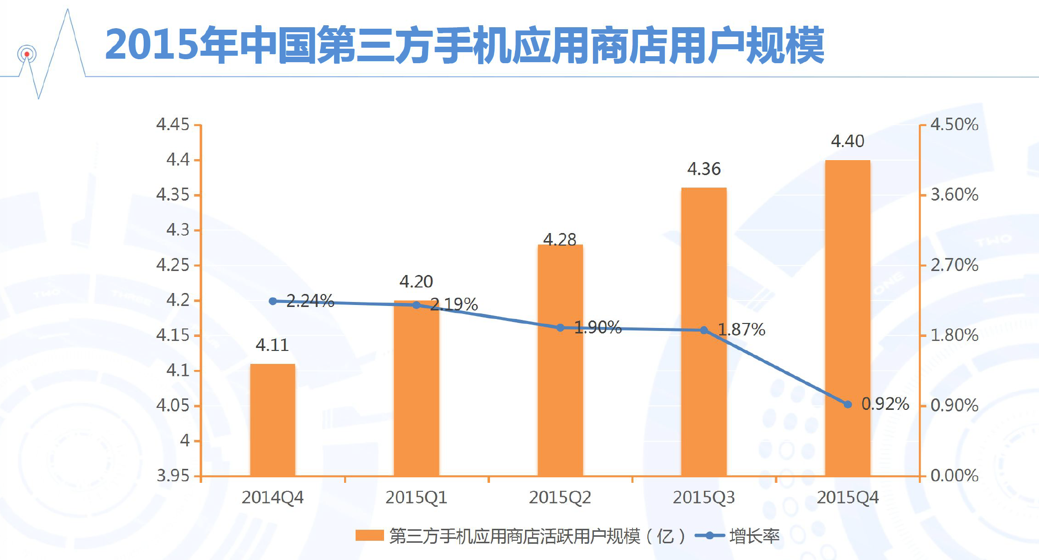
\includegraphics[width=0.9\textwidth]{figure/user-scale.png}
	\bicaption[fig:user-scale]{艾媒咨询《2015-2016中国手机应用商店年度报告》}{艾媒咨询《2015-2016中国手机应用商店年度报告》\protect\footnotemark}{Fig}{Annual Report of China Mobile Application Store}
\end{figure}
\footnotetext{《2015-2016中国手机应用商店年度报告》\url{http://www.iimedia.cn/40366.html}}


\section{面临的问题以及解决方案}
\label{sec:market-prob}
2015年6月,美国网络安全公司NowSecure发布报告称\footnote{新华网:三星手机被曝存安全漏洞 超6亿用户信息存泄漏隐患。 \url{http://news.xinhuanet.com/finance/2015-06/24/c_127945927.htm}},预装在三星Galaxy手机上的SwiftKey输入法在更新后,存在可以被黑客利用的安全漏洞。
被攻击的机器可以允许攻击者控制用户的网络流量,并在手机上留下后门,攻击者可以在手机上执行任意代码。
并且由于SwiftKey为三星预装软件,所以在非root情况下是无法被卸载的。
利用这一漏洞,攻击者可以监控用户的网络,使用受害者手机摄像头、窃听通话等危害用户隐私的行为。
据统计,有超过6亿部三星手机由于该漏洞处于安全威胁之中。


2015年10月19日,苹果公司(由SourceDNA安全公司提供样本)下架了256款App\footnote{新华网:广告公司涉窥隐私 苹果下架众多应用。 \url{http://news.xinhuanet.com/tech/2015-10/20/c_1116881103.htm}},原因是这些App都使用了第三方广告库有米SDK,该SDK调用了IOS系统的私有API获取邮件地址、设备认证信息和路由数据等隐私数据。
根据苹果公司的解释,这些API并不开放给应用使用,有米SDK通过技术手段绕过了App Store的检查,这些使用了有米SDK的应用造成了用户隐私数据的泄露,将无法上架App Store。
由此可见应用的审查对于应用市场是非常必要而且重要的。


中国工信部曾在微博上公布过2015年第三季度问题应用软件名单,其中35款不良应用榜上有名,其中不乏知名大公司千万级用户量的产品,名单上App的主要涉及强行捆绑安装、未经用户同意收集个人信息、恶意“吸费”等问题。

另外,有些违法分子甚至盗用正版应用,并通过技术手段为其增加广告、甚至病毒,最后重新打包发布到应用市场上赚取非法利益。
通过这种技术重打包的应用通常叫做克隆应用。
克隆应用的危害在中国尤其严重。
由于在中国无法使用安卓官方市场Google Play,第三方市场成为了智能手机用户下载应用最主要的方式。
而第三方市场碎片化严重,监管情况不明,导致克隆应用泛滥。
之前研究有对百度应用市场进行检测,12442个应用中有1928个应用为疑似克隆应用,比例超过10\%。可见克隆应用问题情况之严重。

Android的权限机制可以在一定程度缓解恶意应用以及隐私泄露问题。
Android操作系统会在安装应用时告知用户此应用会使用到手机的哪些权限。
比如App需要连接网络或者获取通讯录,开发者要在App中显示申明需要网络权限和读取通讯录的权限。
用户在安装Android App的时候,系统会弹窗描述该App需要获取的权限,用户只有允许才能安装使用。
但是根据相关用户调查,大部分普通用户不会仔细看安装应用时请求的权限。
甚至一些应用商店安装应用时会跳过这个步骤,直接授予App接触敏感信息的权限,由此造成的问题比如一个手电筒应用能够读取用户通讯录的内容非常普遍。
而虽然Android 6.0版本使用了运行时授权, 在应用使用到相对敏感的权限时会提醒用户是否允许应用使用此权限,在一定程度上提高了隐私信息的安全性,但是Android系统版本碎片化严重。
截止2016年5月2日,Android 6.0系统只有7.5\%的装机量,而且动态权限方法无法追踪获取的信息流向,所以并不能完全消除隐私泄露隐患。

市面上有“360手机卫士”,“腾讯手机管家”等工具App查杀Android手机病毒。
通常手机病毒会做些诸如劫持支付软件,记录输入的账号密码,自动发送短信的行为,手机病毒查杀工具可以根据这些行为特征进行静态或者动态的安全保护。

但是这些手机病毒查杀工具对于隐私保护的效果甚微,因为隐私泄露没有明显特征。
例如一个App获取了设备通讯录信息并发送到服务端,查杀工具难以判断这是否是一个恶意的隐私泄露行为,因为诸如微信等App需要通过通讯录信息帮助用户添加好友。
再例如一个App收集用户的手机号码,在发送到服务端的时候不直接将手机号码放在发送的内容中,而是通过发送1次“a”,3次“b”,5次“c”来表示“135”。
这种泄露方式难以发现,Android的用户隐私安全受到了极大的威胁。

以上事例都生动的说明了应用市场需要对开发者上传的应用进行审核。
审核过程包括但不仅限于查杀病毒、分析应用是否具有恶意行为以及检查克隆应用等等。
在进行单应用审计的同时,应用市场还可以综合海量的审计结果,进行分析与预警。
之前轰动一时的XcodeGhost,就是在编译iOS App时向应用代码中注入了恶意的代码,使得App运行是会收集用户的信息并且上传到攻击者的服务器;
之前在研究中发现很多病毒也会伪装成正常的包名来躲避安全分析工具的检查,例如病毒DroidKungFu~\supercite{kungfu}就是在感染的app中伪装成\texttt{com.google.update}(Google的应用更新服务库)。
只要应用市场能够实时监控与分析海量的审计结果,上述病毒的爆发就能即使被发现并制止。

在应用开发中,通常会使用到第三方库。
第三方库为开发者提供一个或一组编写好的功能,加速软件开发。
研究表明第三方库的质量参差不齐,很多广告库会泄露用户的隐私,而最近发生的淘米客和百度SDK事件则更加恶劣,这些SDK中嵌入了远程命令和控制服务器(C\&C服务器),使得目标机器可以接受来自服务器的命令,从而被控制,给外界提供传输恶意命令的平台,危害用户的隐私数据安全。
即便没有恶意,很多第三方库还会存在很多漏洞,这些漏洞也可能将用户的手机暴露在不安全的环境中。
同时使用一些可能导致性能问题的第三方库对应用开发者来说也会造成不小的损失。
所以应用市场可以通过检测应用中是否存在有问题的第三方库,来定位问题库的受害者,并提醒开发者使用经过补丁升级后的第三方库,或者禁止使用有问题的第三方库。

综上所述目前第三方应用市场对应用的审查与分析还比较有限,主要体现在以下三个方面:隐私问题审核、重打包应用检测以及第三方库检测。
本文设计的应用审核系统AppShield旨在提供以上功能的同时保证一定的扩展性,使得应用市场能够更加安全,有效。

针对隐私问题审核,AppShield集成了单应用审查工具AppAudit~\supercite{appaudit},对于单个应用,会使用AppAudit进行分析,检测出隐私泄露威胁;
同时AppShield会结合整个市场的应用检测结果进行进一步分析,得出市场的隐私泄露概要,以及市场上造成隐私问题最多的组件,并对其进行深度分析。

针对重打包应用和第三方库检测,AppShield设计了一种应用相似度检测的方法,可以同时应用与以上两种检测中。
对于每个应用,此方法会进行一次指纹提取,生成应用的指纹信息;
依据指纹信息进行比对,可以得出应用之间的相似度,从而找出潜在的重打包应用;
由于相似度检测的方法是基于应用代码的,所以第三方库可以使用dex工具打包成SDK,通过比对此SDK和应用的相似度,即可知道应用是否包含了这个第三方库。

在检测应用相似度的工作上,最大的挑战就是混淆。
而AppShield中使用的方法能够应对大多数情况的混淆方法,使得系统能够检测出使用了混淆技术的重打包应用,使得检测的广度得到了提高。

\section{本章小结}
\label{sec:intro-conclusion}
本章首先介绍了移动市场繁荣的现状,然后对目前应用市场存在的问题进行了分析与讨论,最后提出了应用市场需要有检测隐私泄露问题、检测重打包应用、检测第三方库三方面的能力,并给出了AppShield解决方案,同时阐述了AppShield多方面的优点。
\chapter{相关背景}
\label{chap:background}
本章将对相关背景进行介绍。~\ref{sec:android-perm}节和~\ref{sec:background-appaudit}节分别介绍了Android权限机制以及单应用审查工具;~\ref{sec:sim-detect}节中介绍了相似度检测;~\ref{sec:obfuscation}节中介绍了Android混淆相关概念以及技术;~\ref{sec:background-conclusion}节对本章进行了小结。

\section{Android权限机制}
\label{sec:android-perm}

Android的权限控制分为几个层面,系统层面和应用层面。
在系统层面,Android是运行在Linux内核之上的,Linux内核已经经过多年广泛的使用,而且很多对安全敏感的环境都在使用Linux。
Linux一直活跃在研究领域,经过数十年的发展与修正,已经成为了一个稳定且安全的操作系统内核。
作为移动计算的基础,Linux内核为Android操作系统提供了很多关键的安全特性:

\begin{enumerate}
  \item 基于用户的权限模型
  \item 进程隔离
  \item 可拓展的安全进程内通信
\end{enumerate}

Linux作为一个多用户操作系统,一个基本的安全规则就是隔离不同用户的资源。
在Linux中,一个用户不能读另一个用户的文件、一个用户不会耗尽另外一个用户的资源,如内存、CPU以及硬件设备等。

Android平台利用了Linux的基于用户粒度的保护这一特点,实现了识别并且隔离不同应用的资源。
在安装应用时,Android操作系统会给应用分配一个独特的系统标识,即Linux的UserID和GroupID。
在运行应用时,Android会让这个应用跑在所述用户单独的进程下。
这跟很多其他的操作系统,包括Linux的传统用法不同,一般的做法都是多个应用会运行在同一个用户下面。

这种做法建立了一个内核级别的应用沙盒,使得不同应用之间的资源通过不同的UserID和GroupID实现了隔离。
由于这个沙盒是建立于内核级别的,无论是应用代码、Dalvik虚拟机还是支持库都无法越权访问属于其他进程(应用)的数据。

其中root为最高权限的用户,可以访问任何权限,在Android中只有内核以及小部分核心系统应用是以root权限运行的。在一般情况下,root权限是不会开放给用户的,这是为了保护用户的root权限不被恶意应用所利用。

在应用层面,默认情况下,一个应用只能访问有限的系统资源,这是为了保护用户的数据以及硬件不被误用或者恶意使用。
Android通过多种方式来实现对应用的限制,有些功能直接不提供API来操作,例如没有Android API直接操作SIM卡。
同时,一些可能会使用重要资源的敏感API只会提供给被信任的应用使用,这种机制就是我们经常说到的权限。

在Android系统中,受到保护的API主要有以下几类:

\begin{enumerate}
	\item 摄像头功能
	\item 位置信息
	\item 蓝牙功能
	\item 通话功能
	\item 短信、彩信功能
	\item 网络连接
\end{enumerate}


这些资源只允许操作系统访问。
如果一个应用想要使用这些资源,必须在Manifest中声明使用对应的Capabilities。
如图~\ref{fig:android-perm},需要监控传入的短信的应用要在Manifest指定声明android.permission.RECEIVE\_SMS。
当安装应用时,系统会弹窗描述该App需要获取的权限,用户只有允许才能安装使用。
如果用户继续安装,系统则会认定用户已经授予了应用使用要求的权限。
用户要么全部接受,要么拒绝安装,用户无法拒绝某一项权限。

\begin{figure}
	\centering
	\begin{lstlisting}[language={xml}]
	<manifest xmlns:android="http://schemas.android.com/apk/res/android"
		package="com.android.app.myapp" >
		<uses-permission android:name="android.permission.RECEIVE_SMS" />
		...
	<manifest/>
	\end{lstlisting}
	\bicaption[fig:android-perm]{AndroidManifest.xml中声明监控接收短信的权限}{AndroidManifest.xml中声明监控接收短信的权限}{Fig}{Using RECEIVE\_SMS Permission in AndroidManifest.xml}
\end{figure}

在Android 6.0版本后加入了运行时授予权限的功能\footnote{Android Permission: \url{https://developer.android.com/training/permissions/requesting.html}},使得用户是在应用运行时向Android授予权限,而不是在应用安装时授予。
此方法可以简化应用安装过程,因为用户在安装或更新应用时不需要授予权限。
同时用户可以准确知道应用会在什么操作时需要什么权限,可以细化权限的使用。

\section{单应用审核工具AppAudit}
\label{sec:background-appaudit}

虽然Android的权限机制能够在应用的使用中有效的展示其使用了哪些敏感资源,但是无法追踪应用是如何使用这些敏感资源的。
以“滴滴出行”应用程序为例,在安装时,系统会弹出提示框描述该应用需要获取的权限.
用户无法授权其中一个或几个权限,只能全盘接受或者不予安装。
如图\ref{fig:didi}所示,用户在安装时被提醒“滴滴出行”应用在运行时需要读取内部存储、拨打电话、读取讯息获得精确位置等权限。
而从权限列表中,用户却无法得知应用是如何使用这些权限,比如应用需要获得短信的原因、应用是否会将用户短信通过网络或者其他方式泄露出去。
这些都给了恶意软件可乘之机,导致用户处于隐私数据泄露的威胁之中。

\begin{figure}
	\centering
	\subfigure[]{
		\label{fig:didi:a}
		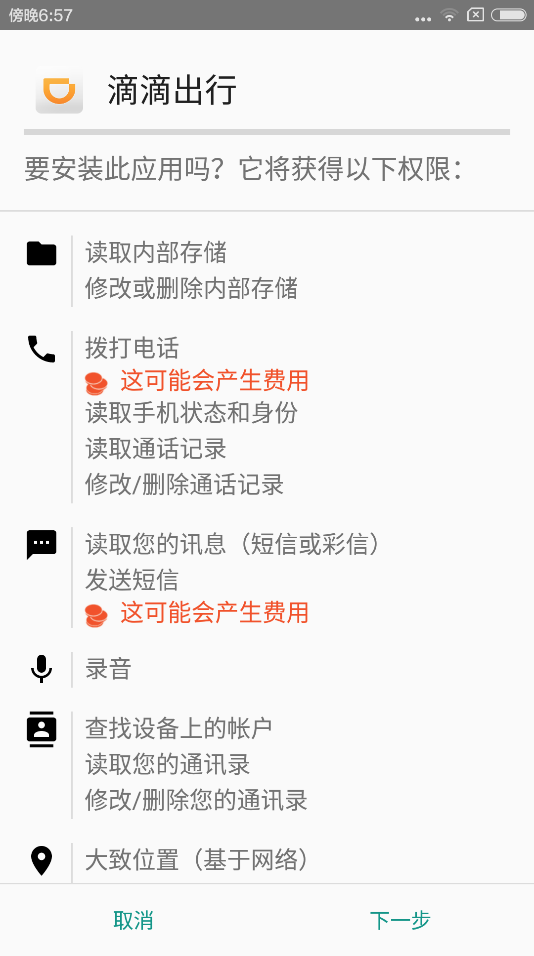
\includegraphics[width=0.4\textwidth]{figure/didi-a.png}
	}
	\hspace{1in}
	\subfigure[]{
		\label{fig:didi:b}
		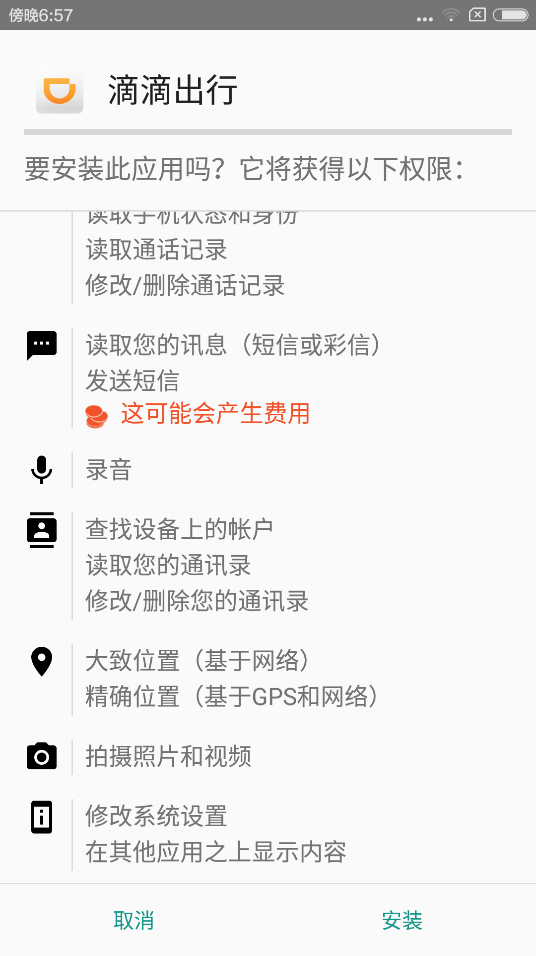
\includegraphics[width=0.4\textwidth]{figure/didi-b.png}
	}
	\bicaption[fig:didi]{“滴滴出行”安装时显示的权限列表}{“滴滴出行”安装时显示的权限列表}{Fig}{Requested Permission List When Installing "DiDiChuXing"}
\end{figure}

为了解决隐私泄露问题,很多应用市场都使用了很多方法来对上传至市场的应用进行审核,从而识别并剔除存在隐私泄露问题的应用程序。
例如,Android在4.2版本中引入了AppVerfiy的服务。
使用了该服务的手机会在安装新应用时,将应用的相关信息,比如应用包名称、SHA-1值等信息提交给AppVerfiy服务器。
服务器会根据这些信息去识别应用是否为已知的恶意软件,最终报告给用户该应用是否会泄露隐私数据。
但由于获得信息有限并且恶意软件发布者可以通过简单的更改包名来绕过检查,所以AppVerfiy的准确率有限~\supercite{appverify}。

在近几年来,很多研究都将程序分析的方法~\supercite{appintent,flowdroid,pios,zhang2013vetting,jiang2013detecting}引入到了移动应用的隐私泄露问题检测中。
这些研究一般分为两种,静态分析和动态分析。
静态分析是指通过对代码进行数据流等方法进行分析,最终找出敏感信息泄露的代码路径。
而动态分析是指在代码运行过程中,通过注入等方法监控程序运行状态,从而在敏感信息泄露发生时将其阻挡。
AppAudit结合了动态和静态的分析方法,分别避免了静态分析内存占用大,分析时间长和动态分析开销大,效率低,覆盖率低的缺点。
AppAudit利用的模糊执行的方法极大程度的减少了分析时的内存占用以及分析时间。
使得AppAudit可以在200多MB、几秒内完成对一个应用的分析。
从图~\ref{fig:appaudit:time}和图~\ref{fig:appaudit:accuracy}中可以看出,AppAudit的分析时间远少于其他同类型工具,同时还能保证比较高的准确率。

\begin{figure}
	\centering
	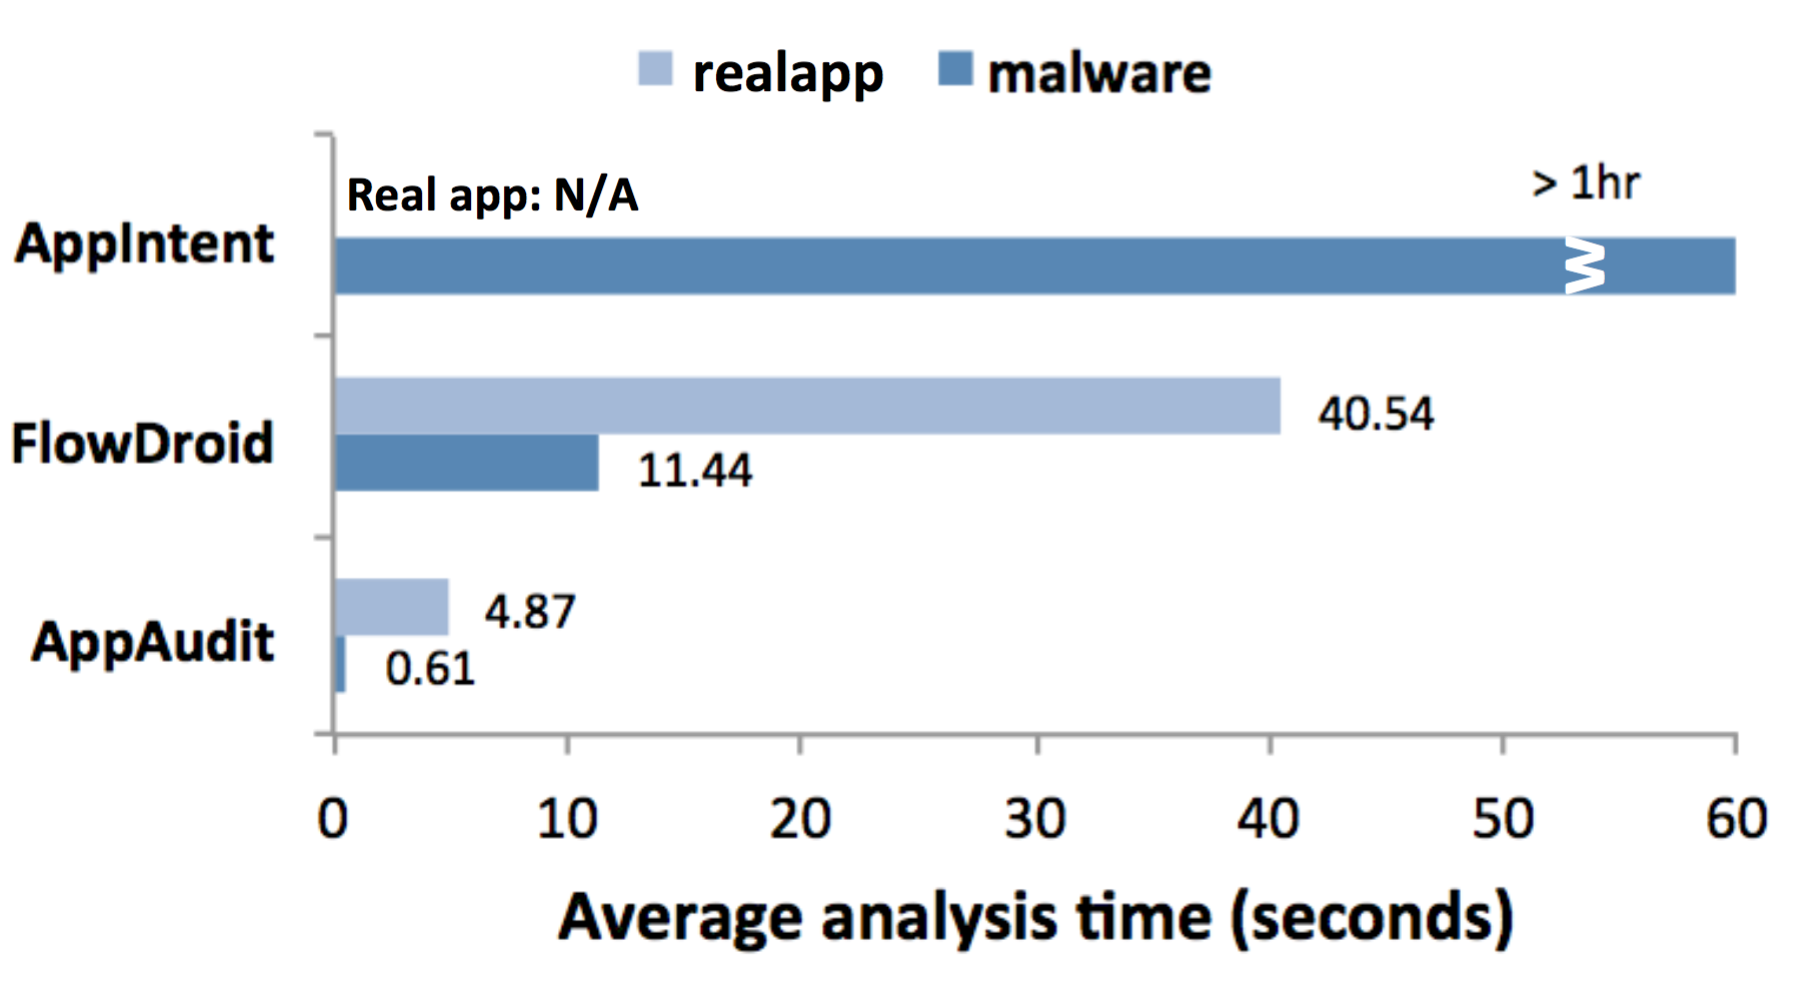
\includegraphics[width=0.7\textwidth]{figure/appaudit-time.png}
	\bicaption[fig:appaudit:time]{AppAudit与其他工具分析时间对比}{AppAudit与其他工具分析时间对比~\supercite{appaudit}}{Fig}{Analysis Time Comparison between AppAudit and Other Tools}
\end{figure}

\begin{figure}
	\centering
	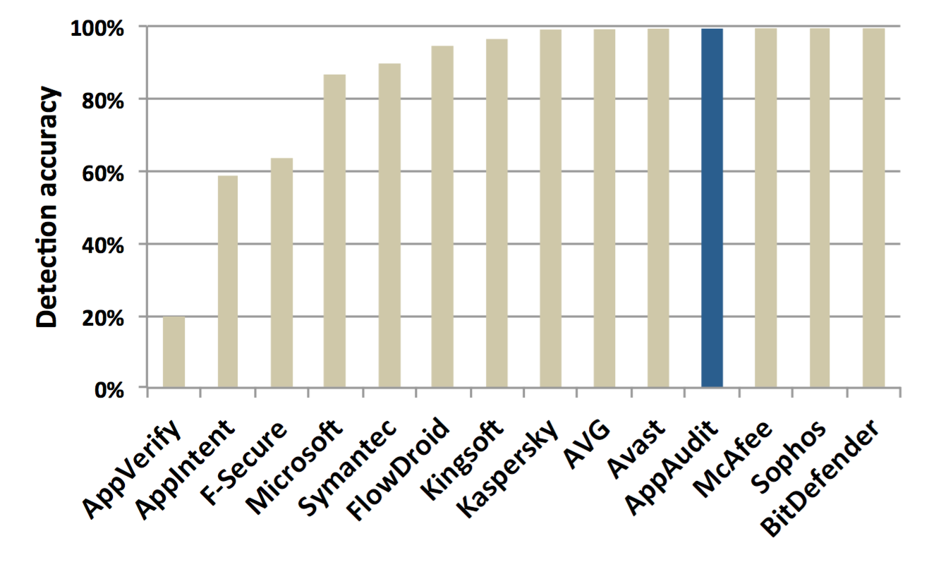
\includegraphics[width=0.7\textwidth]{figure/appaudit-accuracy.png}
	\bicaption[fig:appaudit:accuracy]{AppAudit与其他工具的准确性对比}{AppAudit与其他工具的准确性对比~\supercite{appaudit}}{Fig}{Detection Accuracy Comparison between AppAudit and Other Tools}
\end{figure}

\section{相似度检测}
\label{sec:sim-detect}

第三方库是现代程序开发过程中无法缺少的一部分。
开发者通常会将经常复用的代码以库的形式打包,来加速软件开发,而发布给他人使用的库则成为第三方库。
在Android应用开发中,常见的第三方库种类有工具类库,比如gson,okhttp等、广告类库,如Tapjoy,Admob,还有数据统计类库Google Analytics,TalkingData等等。
由于第三方库的质量参差不齐,开发者使用的第三方库可能会给应用带来相应的隐私问题。
最近研究表明~\supercite{enck:androidsec,grace2012unsafe},很多有名的第三方库会泄露用户的隐私信息。
此外由于第三方库广泛的运用于应用开发中,第三方库占应用代码大多数比例是很常见的情况。
这对Android应用程序分析带来了额外的开销于噪音,所以很多程序分析需要先排除掉第三方库来是的分析过程更高效准确。
例如在检测克隆应用时,需要排除掉第三方库对结果造成的影响。

另外,当在应用审查中,如果不能有效的检测出应用包含的第三方库,那么在应用出现隐私泄露或者安全漏洞时,无法定位。
如今有很多安全相关的分析工具能对应用很多方面进行分析,包括隐私泄露~\supercite{androidleaks, flowdroid, amandroid, droidsafe,rdroid}、权限使用检查~\supercite{remystified}、动态代码加载~\supercite{execute}、SSL/TLS安全相关问题~\supercite{topin, eve}等等。
如果不能在将第三方库和开发者本身的代码区分开,我们就很难确定,存在的问题到底是开发者有意为之还是只是因为引入了一个有问题的第三方库。

第三方库的检测可以通过检测应用与第三方库之间的组件相似程度来实现。
而这种相似度检测的方法也可以应用与克隆应用检测中,如果检测到两个应用相似度很高,并且两个应用的开发者密钥不同的话,这对应用就为一对潜在的克隆应用。

在检测过程中,最大的挑战来自于混淆。
代码混淆是现代软件开发中一个常用的技术,是指将程序代码做一种变形,在不影响程序功能的情况下,使得反编译后的代码难于阅读和理解。
代码混淆能够有效地增加逆向工程的难度,使得软件破解与注入的成本大大增加。
另外在移动应用开发中,代码混淆还能通过将代码中的各种变量名重命名成短名称,来有效的减少应用的代码体积,从而对应用包进行“瘦身”。
而混淆过程中,应用的代码会发生改变,会使得针对应用代码的程序分析变得困难。

\section{Android混淆技术}
\label{sec:obfuscation}

Android应用是使用Java语言进行开发。
使用Java开发的一个主要好处就是可移植性,编译好的程序可以跑在大多数平台上。
Android应用在构建过程中会首先被编译成Java字节码,最终通过Dalvik编译器编译成平台无关的Dalvik字节码,最终运行在Dalvik虚拟机上。
为了节省空间,Java会将所有类型名、变量名和方法名全部存储在常量库中。
而Dalvik在编译过程会把所有Java字节码文件合并压缩成一个Dalvik字节码文件,多个常量库也会合并成一个,从而使得多个类共用的资源只需要存成一份,节约空间。
这些常量库和指令为虚拟机还原Java语义。

由于字节码的语义丰富,已经有很多成熟的反编译软件,例如jd, jadx, dex2jar等等。
经过反编译软件处理后的程序代码已经可以基本上和源代码相同。
这些反编译软件极大程度上威胁了软件作者的权益。
不法分子可以通过反编译来破解软件、加入恶意代码后将软件重新发布等等。

混淆工具是防御反编译威胁的主要方式之一。
混淆会在不改变代码功能的同时,改变代码的形式,使得代码变得更加模糊。
混淆的目标是使得反编译后的程序难以被理解,从而使破解者需要花费更多的时间与精力在混淆代码上。
在混淆中,被混淆的部分成为混淆范围。
在开发中,很多库会指定在混淆中需要将其排除在混淆范围之外,以防未知的错误。
而开发者也有时需要指定某个类或者某个包不需要被混淆,来保证程序的正常运行。

在混淆中最常用的几种方式为标识符重命名、代码缩减、包结构重组织。
值得注意的是,很多混淆器也可以对字节码进行优化。
类的成员方法和成员变量可能会在优化的过程中发生变化,所以字节码的优化也可以被视为一种混淆。
接下来会分别介绍以上所说的这几种常用的混淆技术。

\subsection{标识符重命名}
标识符重命名是最基本的一种方式,在Java语言规范中规定到,一个Java程序的标识符包括:
\begin{itemize}
	\item 包
	\item 类型(类或者接口)
	\item 值域
	\item 方法
	\item 参数(方法参数、构造函数参数或者exception handler)
	\item 本地变量
\end{itemize}

但是并不是所有的标识符在编译之后都会保留在字节码中,参数和本地变量可能会在编译的过程中转化成本地变量数组的内存地址。
如果是在调试模式下编译字节码的话,参数和本地变量的名字就会保留在字节码中的LocalVariableTable中。
虽然去除掉LocalVariableTable也会使得反编译变得更困难,但是一些先进的反编译器已经可以自动推测参数以及本地变量名,既然无法阻止自动推测,那么在LocalVariableTable中的名字就不需要被混淆选中进行重命名。
所以只有前五种标识符会被混淆进行重命名。

另外,也并不是所有标识符都能被重命名的。
Dalvik虚拟机在运行时是动态加载并链接引用类型的。
之前提到类名、方法名都是位于字节码的常量池中。
因此,只有在混淆范围内使用的标识符能够被重命名。如
果标识符在混淆范围外的代码中被使用,那么此标识符就不能够被重命名,例如一些类库和标准库。
除此之外还有以下四类标识符是不能被混淆的:
\begin{enumerate}
	\item 实现了某个在混淆范围外的父类或者接口的纯虚方法的方法
	\item 重写了某个在混淆范围外的父类的方法
	\item 开发者指定的不被混淆的标识符
	\item 充当回调函数的方法
\end{enumerate}
当一个应用被反编译后,破解者不仅仅是从标识符的名字来理解标识符所代表的意义,标识符的上下文同时也能反映出一定的信息。
在重命名标识符时,混淆器会充分利用重载来复用标识符的名字,并且会根据字典序来顺序的为标识符重命名,使其成为无意义的名字。
经过重命名后,破解者只能通过代码的上下文来猜测标识符所代表的意义,从而使得破解者理解代码的过程更加困难。
在混淆时一个额外的好处就是字节码的体积会因为更短的标识符名字和标识符名字的复用而减少。

在Java应用中,一个应用时由一个或多个包组成的。
包的作用是组织类,一个包中包含零个或多个类、接口或者子包。
另外包也决定了类的命名空间,包采用树形的存储方式,在一个包中的类、接口和子包的名字不能相同,但是在不同包中的类、接口或者子包,名字可以相同。
通过字典序来顺序生成标识符名字为混淆的一个功能,而顺序生成的步骤会在每个包中重新开始。

根据以上规则,混淆器会对混淆范围内所有可以被混淆的标识符进行重命名,并且在顺序生成标识符的过程中,会在不同包内尽可能的重用标识符的名称。
另外混淆器会充分利用重载来重用标识符,来同时达到混淆代码以及节省空间的作用。

\subsection{代码缩减}

在应用开发中,实际运行的代码可能只是总代码的很小一部分。
特别是在开发者引入了一些第三方库时,这个情况非常常见。
因为第三方库通常会提供一组或多组程序功能,而在开发中可能只会用到其中的小部分。
所以第三方库的代码就会存在大量的冗余,导致代码体积不必要的增大。
在很多混淆器中,也会提供代码缩减的功能。
代码缩减是指把代码中未被调用的方法,和未被引用的类移除,从而减少代码体积,节省空间。

\subsection{包结构重组织}
通常,提供一组相同功能的类和接口会被组织到一个包中,以便于类的查找和使用。
开发者通过包的结构来组织程序的构成。与此同时包结构也会给破解者提供信息来分析字节码。
破解者在理解了包中的一些类后,理解同一个包中其他类就变得更加简单了。

包的另外一个作用是控制包内成员的可访问性。
一个类T中的成员如果被声明为protected,那么只有和T在同一包中的类型和T的子类型能访问此成员。
如果一个类T中的成员没有声明访问类型(默认情况下),那么只有在和T在同一包中的类可以访问其成员。

包结构重组织会打乱原本的包结构,把一些包或者类重新组织到新的包或已有的包中。这样破解者就没法利用包结构这个信息来理解程序从而进行破解。
但重新组织包结构可能会带来一定的副作用,比如破坏原来的包访问权限,因为对包进行了重新组织,一些类或者类中成员的可访问性拓宽。
庆幸的是,扩充字节码的访问范围并不会影响字节码中的指令,从而不会对程序的行为造成影响。

\subsection{字节码优化}

\begin{enumerate}
	\item 死代码移除
		在代码缩减过程中,已经会移除掉没有被调用的方法以及没有被使用的类。
		然而在代码缩减处理后保留下来的方法和类中还会存在着没有被执行的代码。
		优化器可以利用分析变量的活性来判断代码是否真的需要被执行。
		如果一个函数调用没有使得调用的类状态发生改变,我们称这个函数调用是没有“副作用”的。
		如果一个没有“副作用”的函数调用返回值没有被使用,此时这个函数调用也会被移除。
	\item 接口和类合并
		在很多混淆器中,会通过减少类和接口的数量来减少类的数量从而减少代码体积。
		把多个接口合并成一个可能会使得只实现单个接口的类变得不完全。
		这在Java语言层面是不合法的。
		在Java语言规范中提到,除了abstract类,其余类的所有继承的接口的abstract方法必须被实现,无论是在此类或是在此类的父类中。
		但是根据Java语言规范中的二进制代码兼容性章节所述,向一个接口中添加一个abstract方法不会破坏已有二进制代码的兼容性,所以接口合并这种优化方法是可以应用在字节码层的。
	\item 其他
		混淆器可能还会用到一些其他的代码优化技术,比如移除未使用的参数,改变类和方法的访问权限等等。
\end{enumerate}

\subsection{本章小结}
\label{sec:background-conclusion}

在本章中主要介绍了在本论文中用到的相关技术与背景,其中包括四大部分,第一部分介绍了Android的权限机制;第二部分介绍了本论文使用的单应用审查工具AppAudit;之后第三部分介绍了相似度检测相关背景;最后介绍了在相似度检测中遇到的挑战,混淆的相关知识。
\chapter{相关工作}
\label{chap:related-work}

本章将对相关工作进行介绍,在AppShield牵涉的领域,已有若干学者有一定的研究与成果,本章主要阐述已有的相关工作以及其优缺点。
~\ref{sec:related:privacy-protect}节、~\ref{sec:related:clone-app}节、~\ref{sec:related:third-lib}节分别介绍了Android隐私保护、克隆应用检测以及第三方库检测的相关工作,~\ref{sec:related:conclusion}节对本章进行小结。

\section{Android隐私数据保护}
\label{sec:related:privacy-protect}

近年来,除开AppAudit之外,也有很多研究将程序分析的方法引入Android隐私数据保护领域中。

AppIntent~\supercite{appintent}使用的是符号执行的方法对应用进行静态程序分析,它对传统的符号执行进行了优化,通过建立Android生命周期的模型,有效的减少了代码的执行路径。
即便如此,AppIntent在16核的机器上分析一个应用的时间仍然长达数十分钟,有的甚至超过了一个小时。
AppIntent另外一个缺陷就是内存占用过高,在分析中,AppIntent经常会占用内存高达32GB,这在个人计算机上是很难应用的。

FlowDroid~\supercite{flowdroid}利用了Soot注入框架~\supercite{soot}实现了对Android应用的静态污点分析。
FlowDroid通过使用Dexpler将应用的dex代码转换成Jimple三地址码。
然后通过建立函数调用图,最后进行污点分析。

TaintDroid~\supercite{taintdroid}通过修改Android中的Dalvik虚拟机,实现了动态的污点分析功能,能让用户在运行时追踪手机敏感信息的走向。
但是TaintDroid会在运行是带来14\%的开销,这对用户使用手机影响较大。

\section{克隆应用检测}
\label{sec:related:clone-app}

DroidMoss~\supercite{droidmoss}利用模糊哈希(Fuzzy Hashing)的方式来检测重打包应用。
模糊哈希是一种能应对内容增减的哈希方法。
它首先将字节码进行稳定化,去除易变的寄存器,只保留相对稳定的操作数(opcode);
另外它将哈希内容分段,同时利用滚动哈希的方法,使得在哈希内容发生增减时,只有增减前后的哈希段会有差异,因此能使用相似哈希段占总共哈希段数的比例来判断应用是否为重打包应用。
此方法的好处在于对于一个应用只需要一次模糊哈希,比对时只需要比对哈希结果,另外对于两个有序列表的共同元素查找的复杂度不高,可以接受。
缺点是此方法依赖于字节码的稳定性,虽然模糊哈希已经对字节码进行了处理,但是字节码操作数在混淆中发生变化的情况不是非常罕见。
所以在针对混淆应用的检测时,漏报率可能比较高。
另外此方法是基于两两比较,所以当需要处理海量应用时,扩展性较差。

JuxtApp~\supercite{juxtapp}使用类似的字节码处理方法,保留操作数,对处理后的字节码使用k-gram和基本块进行分段,并对分段后的字节码进行特征哈希,最后通过对比应用的特征向量来判断应用是否有相似部分。
不同的是,JuxtApp主要针对的是识别存在问题代码的应用。

WuKong~\supercite{wukong}通过两阶段检测来识别克隆应用。
WuKong在第一阶段会简单计算出不同Android API调用的次数,将提取出的向量进行编辑距离的计算,只有低于阈值的应用对才会进行下一步的检测。
由于市场上大多数应用都不是克隆应用,所以在这一步可以剔除大量的非克隆应用。
在第二步中,WuKong将对应用进行基于Boreas~\supercite{boreas}的代码克隆检测方法。
在这一步中,将详细的计算代码的特征并进行比较,最终得出潜在的克隆应用。
WuKong对简单的标识符重命名的混淆应用是有效的,但是由于WuKong会依赖于具体的代码(例如Android API调用),所以当代码发生变化时,比如代码发生缩减或者由于代码优化,Android API调用被剔除,检测会失效。

\section{第三方库检测}
\label{sec:related:third-lib}

在克隆应用检测的研究中,通常需要剔除掉第三方库来增加检测的准确性,之前的很多研究~\supercite{grace2012unsafe,book2013longitudinal,chen2014achieving,stevens2012investigating,shekhar2012adsplit}都是通过设置白名单的方式来进行第三方库的检测。
研究者通过经验或者数据总结出使用较多的第三方库,把这些第三方库的包名记录进白名单。
在进行程序分析的时候,来比对代码中是否存在对应白名单中的包名,把出现在白名单中的包名排除分析内容,从而增加准确性。
这种直接的方式好处在于效率高,并且实现简单;
但是这种做法需要长期维护第三方库的白名单,并且由于白名单的比对依赖于包名,所以当应用发生混淆,则白名单就会失效。
所以利用白名单进行第三方库检测在第三方库迭代更新快并且在混淆环境下会失效。

LibRadar~\supercite{libradar}利用聚类的方法,对应用进行第三方库的检测。
LibRadar会计算出应用不同Android API调用的次数,将其提取出特征向量。
然后使用此特征向量进行聚类分析,最终把分析得出的集群识别为第三方库。
由于LibRadar是使用Android API当做特征,所以只能应对标识符重命名的混淆技术,当代码缩减或者由于代码优化,Android API调用被剔除时,检测会失效。

LibScout~\supercite{libscout}利用对应用代码进行指纹生成与比对,来对应用进行第三方库检测。
但由于LibScout在指纹比对时是以类为粒度,并且在比对时使用了包结构的信息,从而当应用因为代码缩减或者代码优化导致应用的方法被移除和当应用使用了包结构重组织的混淆方法时,检测会失效。

\section{本章小结}
\label{sec:related:conclusion}

在本章中,我们对Android隐私保护、克隆应用检测以及第三方库检测的相关研究工作分别进行了阐述,并总结了不同研究各自的优缺点。
对于Android隐私保护,目前的研究除了AppAudit之外,其余的方法在准确性、分析速度、内存占用等方面不能满足大规模应用审查的应用场景;
对于克隆应用与第三方库检测,相关研究工作都无法应对混淆或者只能应对简单的标识符重命名的混淆技术,其他混淆技术如包结构重组织、代码缩减等均会令检测失效。
\chapter{AppShield系统}
\label{chap:appshield}

本文对大规模应用审查系统进行了设计,并实现了原型系统AppShield。
本章将对AppShield系统进行详细的介绍。
在~\ref{sec:appshield:overview}节中,我们对AppShield的工作流程进行了简单介绍;
在~\ref{sec:appshield:collection}节中,我们将介绍了AppShield中应用文件收集的两个方式;
在~\ref{sec:appshield:file-analyze}节中,我们介绍了AppShield中使用的文件分析器Apkinsight;
而AppShield的核心,问题组件分析以及相似度分析将分别在~\ref{sec:appshield:comp-analysis}节和~\ref{sec:appshield:sim-analysis}中介绍。
最后在~\ref{sec:appshield:conclusion}节中,我们将对本章内容进行小结。

\section{AppShield工作流程}
\label{sec:appshield:overview}

AppShield系统主要分为两个部分,采集部分主要目的是持续获取APK文件,分析部分目标是在搜集到的APK里自动找到有隐私问题的应用,自动总结隐私泄露的规律,并且对有问题组件进行进一步的分析。
同时AppShield还会基于相似度检测的方法对应用进行第三方检测以及克隆应用检测。
如图~\ref{fig:appshield-overview}所示,AppShield采集部分通过两种方式获取安卓应用APK文件,一方面系统有一个长期运行的爬虫程序,从多个应用市场获取最新的应用,另一方面AppShield通过合作的形式,从appaudit.io获得样本进行分析。
appaudit.io允许用户上传应用并使用AppAudit进行分析,并将检测结果呈现给用户,AppShield可以从appaudit.io后台获取用户提交的应用APK文件,收集到的APK文件存入AppShield的文件数据库中。
同时,从市场或者用户方面获得的APK文件的元数据(例如下载量、文件名等等)也将自动进入数据库。

\begin{figure}
	\centering
	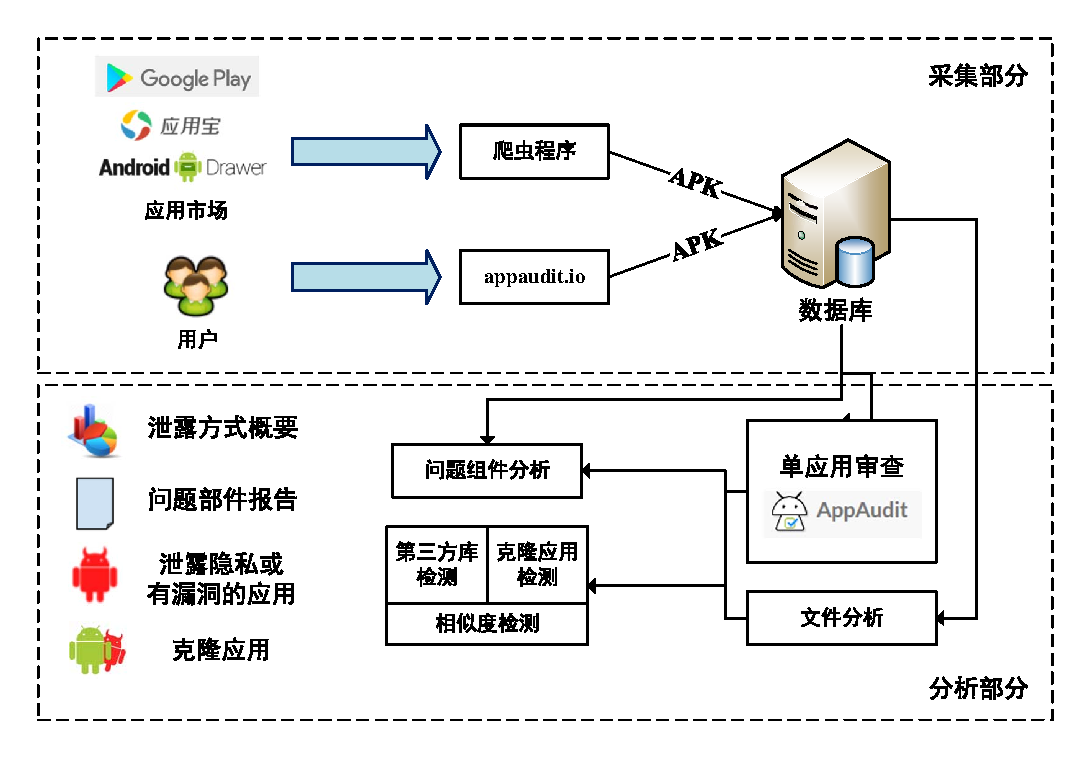
\includegraphics[width=1\textwidth]{figure/appshield-overview.pdf}
	\bicaption[fig:appshield-overview]{AppShield系统架构图}{AppShield系统架构图}{Fig}{Overview Architecture of AppShield}
\end{figure}


AppShield分析部分开始先对数据库中每个APK进行文件分析,提取APK文件中提取App信息(例如应用的名称、识别名、版本、代码中每一个类名等等),放入数据库。
然后(并行地)由AppAudit进行的单App隐私审查,标志出每个App中可以识别的隐私问题。
文件以及AppAudit分析的结果会被用于启动“问题组件分析”,用于找到应用中造成隐私问题的组件,并确认其版本,输出统计结果、问题组件的报告(包括关键样本等)。
另外AppShield提出了一种基于指纹的相似度检测方法,该方法可以应用与第三方库检测和克隆应用检测中。
AppShield会利用此方法对应用进行第三方库和克隆应用检测,最终检测出具有隐私问题或漏洞的应用以及克隆应用。

AppShield系统选择MongoDB作为数据库储存应用元数据。
首先,MongoDB自身拥有性能优秀、可靠性高、社区支持良好的有点。
其次,更重要的是,AppShield系统中的数据交换都使用JSON格式;
JSON格式不仅易于人类阅读和编写,也十分适合机器解析和生成,被广泛接受和使用。
而MongoDB中的数据以BSON(一种JSON的二进制表达和扩展)储存,所以JSON格式与MongoDB天然地相适应。
AppShield系统将应用APK文件储存在共享文件系统而不是数据库中。
每个APK文件有相应的SHA1值,方便查找和去重,并且优化APK在真实文件系统上的存储(文件名统一长度,目录层次完整)。

\section{应用文件收集}
\label{sec:appshield:collection}

应用文件主要来自于两个方面:爬虫程序和appaudit.io网站用户上传。

\subsection{爬虫程序}

AppShield系统的爬虫程序会不断从各个应用市场抓取应用的网页数据信息和APK文件,分别存储在数据库和共享文件系统中。
目前爬取的应用市场覆盖国内外的知名Android应用市场,详细情况见测试与评估部分的测试集。

在设计和实现爬虫程序时,有以下的要求以及实现考虑:
\begin{enumerate}
	\item 全自动的:
		给与一个或多个初始链接,爬虫程序能根据当前网页信息不断地生成下一个目标链接,最终能尽量覆盖整个应用市场。
	\item 同一应用的不同版本:
		在应用发布新版本后,爬虫程序要能及时将新版本的网页信息和APK文件抓取下来。
		在实现中,我们的爬虫会不断地重复扫描应用市场,根据网页上的应用发布日期、应用版本等信息,判断是否发生版本更新,并将新版网页数据和APK文件抓取下来。
		这样,我们就将一个应用几乎所有的版本保存在我们的数据库中。
	\item 容错性:
		爬取一个应用可能持续几分钟的时间(取决于当前网络状况和目标文件大小),而中途可能发生错误和故障,包括网络中断、网页出现404、爬虫程序被意外中止等。
		在实现中,我们将“爬取一个应用”视为一个事务,将“APK文件写入磁盘和网页数据写入数据库”作为这个事务的提交标志。
		通过这种方式,爬虫程序保证原子性和一致性:当错误发生后,已提交事务一定正确完成,未提交事务在未来再次遇到时会被重做。
	\item 并行性:
		应用市场的应用数量非常多,单线程爬虫无法有效地下载大量的应用。
		爬取不同应用本质来说是相互独立的,利用之前提到的基于消息队列的任务调度,爬虫程序很容易实现良好的并行性。
		除此以外,在实现中,利用上述的事务机制,我们保证同一个应用的同一个版本只会被成功提交一次。
\end{enumerate}


结合上述需求,我们以腾讯应用宝上微信应用的抓取为例,介绍一下爬虫的工作流程。
首先,爬虫程序会从腾讯应用宝获取各个分类下的热门免费应用列表,将它们作为初始链接加入爬虫程序的任务队列。
如图~\ref{fig:myapp-pop}所示,这是全部软件分类下的热门免费应用列表,列表中的微信会被作为初始链接添加进任务队列。
随后某个爬虫实例从任务队列中接受这个微信抓取任务,这时可以看作一个事务的开始。
爬虫实例先获取微信应用的HTML文档,如图~\ref{fig:wechat-detail}所示,页面包含大量有用的原始数据,例如评分、评论、下载量等等。
爬虫程序通过CSS选择器和DOM操作,准确定位这些元素,提取其中文本作为原始数据。
这时,爬虫程序会根据这些原始数据判断应用是否为免费应用、应用版本是否还未爬取过(是否有版本更新)。
通过这些判断后,爬虫程序开始下载APK文件。
下载完成后,再次确认APK文件没有重复,并将APK文件储存在共享文件系统中。
最后,网页原始数据被写入数据库,意味着这个微信抓取事务的提交。
如果之前任意一步出错,由于数据库中没有微信的原始数据,下一次遇到微信任务都会重新开始。
另外,页面中还包括了微信的相似应用链接和同开发者应用链接,这些链接会作为新的任务加入爬虫队列,加之初始链接来自于不同种类,保证了爬虫自动覆盖整个市场。

值得注意的是,对于Google Play,我们不能从网页上获取到应用APK文件的URL,因而我们无法简单地直接下载应用APK文件。
幸运的是,许多开发者都为Google Play提供了非官方API和下载模块。
在本系统中,我们使用 Akdeniz 开发的google-play-crawler,作为Google Play的下载器。它对非官方API进一步封装,我们只需提供应用的包名,它便开始查询并下载应用。

\begin{figure}
	\centering
	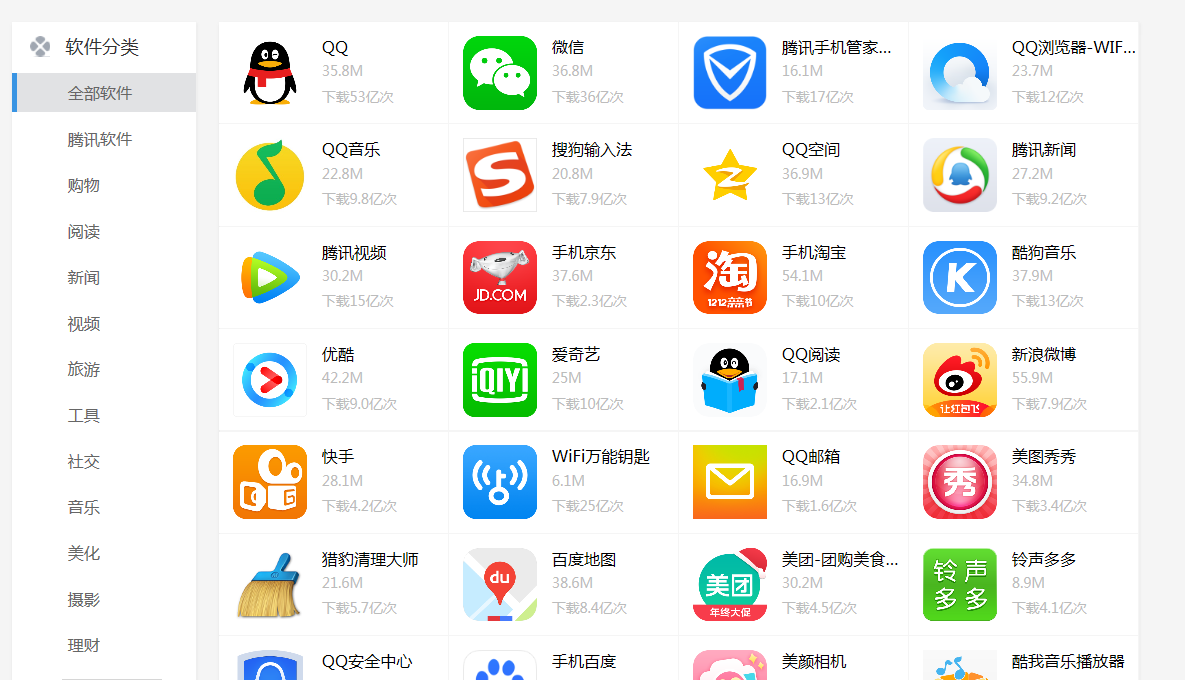
\includegraphics[width=0.8\textwidth]{figure/myapp-popular.png}
	\bicaption[fig:myapp-pop]{腾讯应用宝热门应用页面}{腾讯应用宝热门应用页面}{Fig}{Most Popular Apps in Tencent Myapp}
\end{figure}

\begin{figure}
	\centering
	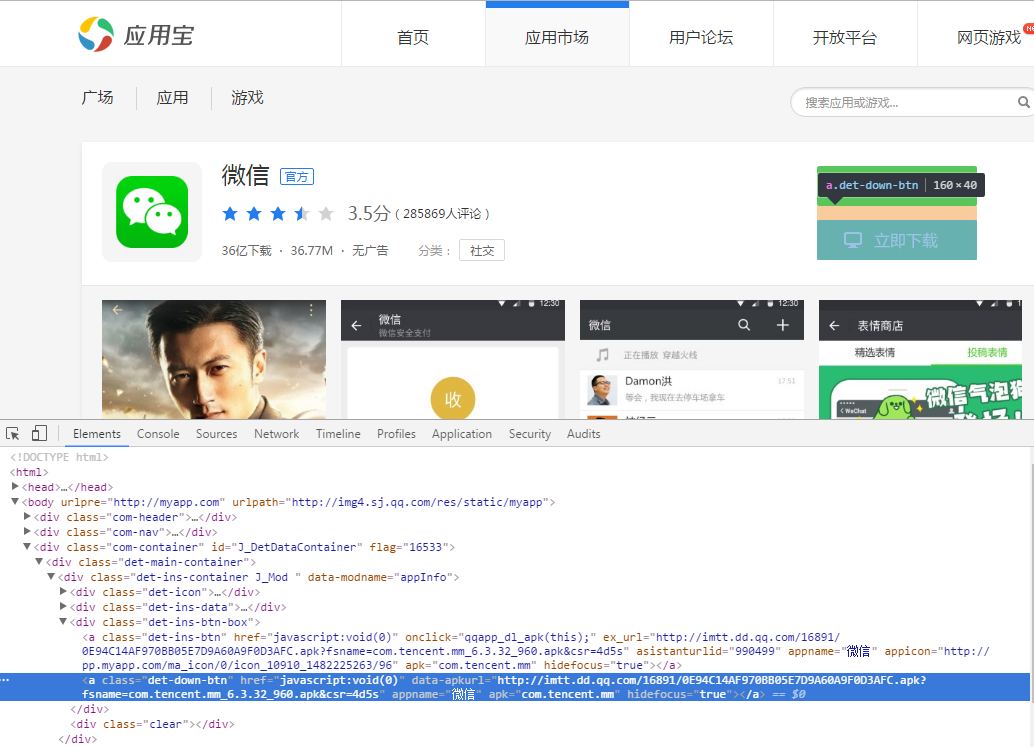
\includegraphics[width=0.6\textwidth]{figure/wechat-detail.png}
	\bicaption[fig:wechat-detail]{微信在应用宝中的详细页面以及下载链接}{微信在应用宝中的详细页面以及下载链接}{Fig}{Detail Info Page of Wechat in Myapp}
\end{figure}


\subsection{appaudit.io用户上传}

appaudit.io网站为用户提供了使用AppAudit的网站接口。
网站访问者可以上传APK文件进行审查,审查之后,网站会显示应用的检测结果。
检测结果包含了应用的基本信息,如应用名、报名、版本、Google Play评分以及应用的隐私泄露行为情况和危险权限使用情况。
图~\ref{fig:appaudit-sample}为appauditio检测出用户提交程序有恶意行为。

\begin{figure}
	\centering
	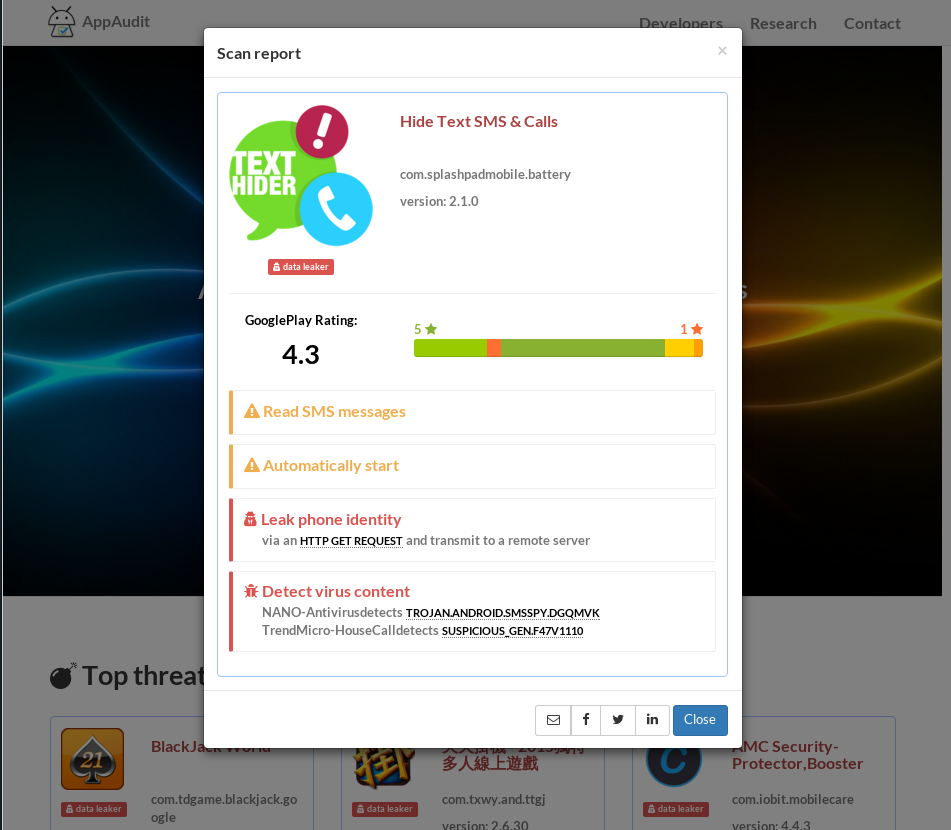
\includegraphics[width=1\textwidth]{figure/appaudit-sample.png}
	\bicaption[fig:appaudit-sample]{微信在应用宝中的详细页面以及下载链接}{微信在应用宝中的详细页面以及下载链接}{Fig}{Detail Info Page of Wechat in Myapp}
\end{figure}

\section{文件分析}
\label{sec:appshield:file-analyze}

在AppShield系统中,由于多个过程都需要对应用SDK进行分解并解析元数据,所以我们开发了Apkinsight文件分析器。
Apkinsight会对数据库中的APK文件进行初步分析,然后将提取整理后的APK元数据以规范的JSON格式输出并储存在数据库中。
Apkinsight分析提取的应用信息如表~\ref{tab:apkinsight}所示。


\begin{table}
	\centering
	\bicaption[tab:apkinsight]{Apkinsight文件分析器分析结果}{Apkinsight文件分析器分析结果}{Table}{Analysis Result of File Analyzer Apkinsight}
	\begin{tabularx}{\textwidth}{|c|c|X|}
		\hline
		提取信息分类 & 提取的信息 & 样例数据\\
		\hline
		应用基本信息 & 包名 & ["\texttt{com.tencent.mm}"]\\
		& 版本名 & \texttt{6.1.0.66\_r1062275}\\
		& 版本号 & 542\\
		& 安装包大小 & 21 MB\\
		& 权限列表 & ["\texttt{com.tencent.mm.permission.READ}"]\\
		& 安装位置 & /data/qq.apk\\
		\hline
		应用证书信息 & 开发者公钥及公钥指纹信息 & ...\\
		& 证书签名是否通过验证 & True\\
		\hline
		应用代码信息 & 代码是否混淆 & True\\
		& 类名列表 & ["\texttt{com.example.MainAcitivity}"]\\
		\hline
		应用内文件信息 & 文件路径 & res/1.jpg\\
		& 文件类型 & jpeg\\
		& 文件大小 & 14KB\\
		\hline
	\end{tabularx}
\end{table}


Apkinsight利用并整合了多种现有的工具,其中包括apktool、JDK中的keytool、jarsigner、baksmali等等。
APK是Android系统使用的应用包格式。
在Android应用构建时,首先应用代码会被编译成Java字节码,之后于Android框架jar包、类库jar包合并打包成classes.jar。
然后Dalvik编译器dx会把jar编译成Dalvik的字节码classes.dex。
然后apk打包器会将应用所用的资源以及Android描述文件AndroidManifest.xml进行二进制化,最后与dex代码、本地库等文件一起打包压缩成APK格式。
值得注意的是,此时生成的APK是未经过开发者签名的APK。
根据Android文档,只有经过签名的应用才能被安装\footnote{App Signing: \url{https://developer.android.com/studio/publish/app-signing.html}}。
对于一个Android应用开发者,需要为自己的应用生成一对公/私钥。
在对应用进行签署的过程会在META-INFO文件夹中生成三个文件MANIFEST.MF、CERT.SF、CERT.RSA。

其中MANIFEST.MF是应用的摘要文件,是利用SHA1对所有非文件夹非签名文件的文件进行哈希,然后通过BASE64进行编码。
这是一个简单的完整性验证,如果攻击者简单修改了程序而未修改此摘要信息,则在安装时会被发现,从而禁止安装。

CERT.SF是应用对摘要的签名,在签署过程中,会使用应用开发者的私钥对之前生成的MANIFEST.MF进行签名,此签名可以用私钥对应的公钥进行验证,从而验证应用开发者的身份。
所以即使攻击者在修改了程序代码的同时重新生成MANIFEST.MF,也无法经过此步的验证。

CERT.RSA中保存了应用开发者的公钥,在应用被安装时,系统会解析出应用的公钥,对CERT.SF进行验证,来验证应用开发者的身份,从而保证用户手机的安全。

Apkinsight的设计动机之一便是在于现有工具过于零散,例如对于应用证书的采集分析,我们会用到keytool、jarsigner、openssl等多个程序。
面对数量巨大的应用以及纷繁复杂的分析工具,研究者需要面对“使用何种工具”以及“如何使用”的困扰,无法专注于应用信息的处理。
Apkinsight对这些工具进行整合封装,为研究者提供统一的工具抽象,提供应用的基本元数据。

在Apkinsight中,会先使用apktool对apk进行解压并且对二进制化的资源文件进行反序列化,之后会使用baksmali将apk的dex代码文件反编译成smali格式以便之后更深度的分析。
同时Apkinsight会利用keytool、openssl以及jarsigner提取出应用的公钥以及公钥指纹信息,并且对应用的签名进行验证。
之后Apkinsight会解析应用的AndroidManifest.xml获取应用的元信息,并且对应用内文件进行遍历,进行信息收集。
最终会将Apkinsight提取整合过的元数据以规范的JSON格式储存在数据库中。
目前,应用元数据没有一种统一的定义与格式,为分析工作带来许多不便。
Apkinsight通过统一元数据格式,为之后的分析工作提供格式化信息

值得注意的是,Apkinsight提供了检测代码是否经过混淆的功能,是通过检测应用的本身包中是否包含Android资源类R来判断应用是否被混淆,关于判断的详细过程,会在~\ref{sec:appshield:proguard}节中进行详细介绍。

\section{问题组件分析}
\label{sec:appshield:comp-analysis}

Android应用数以亿计,质量参差不齐,其中也不乏有很多伪装成正常应用的病毒。
在正常应用中也可能包含各种各样的漏洞。
这些问题应用的源头往往存在于一个组件中,我们称这样的组件为问题组件。
一个组件是由一个包及其所有子包组成,一个存在安全漏洞的第三方库、一个泄露隐私的广告库或者一个伪装成正常包的病毒都是一个问题组件。
问题组件的来源可以有很多地方。
AppShield使用的单应用审查工具AppAudit的审查结果、第三方库的漏洞声明、病毒库都可以成为问题组件的来源。
在应用市场中,这样的问题包可能存在于很多应用中,当我们发现一个问题组件后,如何找出问题组件的“感染”应用,是在本节需要解决的问题。

我们在应用收集阶段,一共获得了116672个应用,其中37095是被检测出混淆的,占总体的31.8\%。
可见未混淆应用占了大部分比例,但是混淆应用也不能忽略不计。
所以针对混淆应用和未混淆应用,AppShield有着不同的处理方法。
对于未混淆应用,我们可以利用文件名、代码等信息来对问题组件进行识别,并对问题组件进行分析。
而对于混淆应用,这些信息都有可能在混淆过程中发生改变,所以需要设计更加稳定的方法来对问题组件进行检测。
对于混淆应用的处理方法,我们会在下一节中介绍。


\begin{figure}
	\centering
	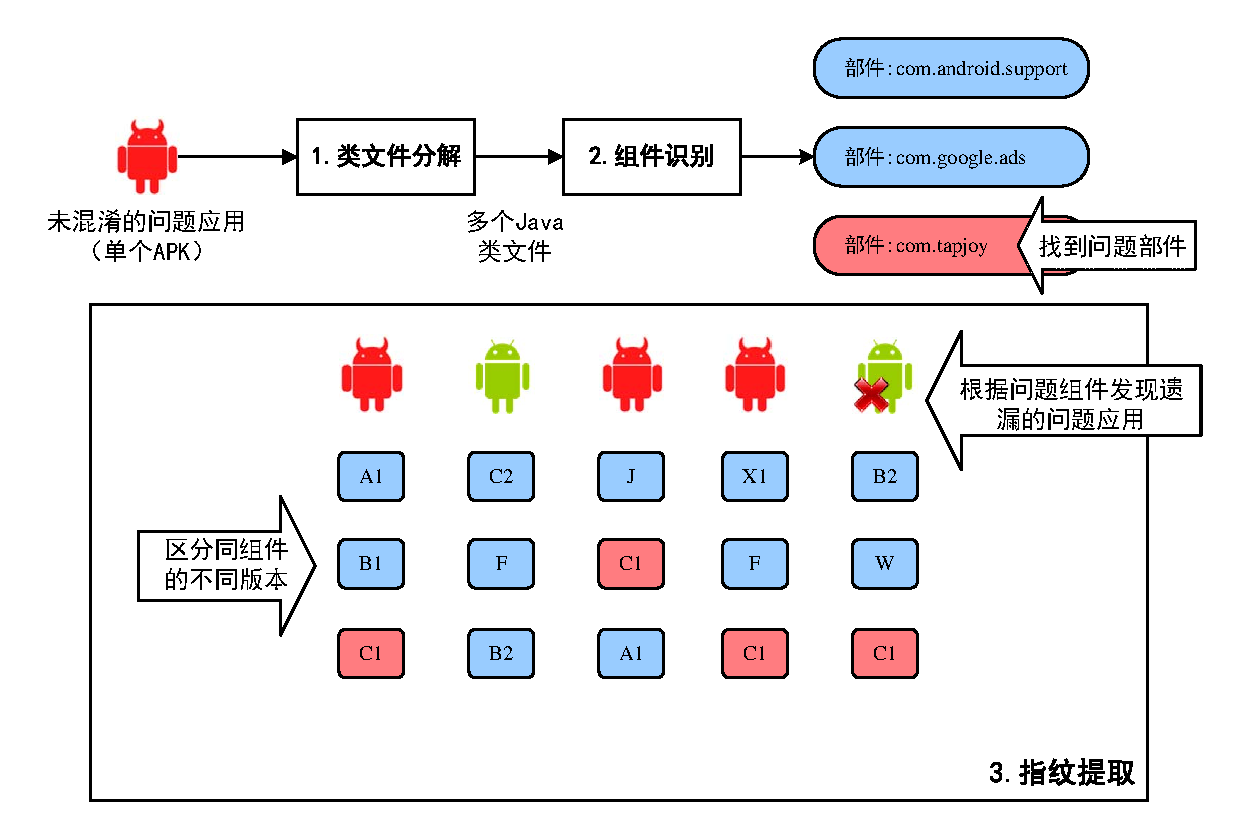
\includegraphics[width=1\textwidth]{figure/comp-analysis.pdf}
	\bicaption[fig:comp-analysis]{问题组件分析主要分析过程}{问题组件分析主要分析过程}{Fig}{Analysis Process of Problematic Components}
\end{figure}


如图~\ref{fig:comp-analysis}所示,在问题组件以及比对应用都未被混淆的情况下,AppShield的问题组件识别会进行以下三个步骤:

\begin{enumerate}
	\item 类文件分解:
		一个应用程序的代码将会按照Java类进行更细粒度的分割,每一个Java类文件中包含代码以及类的成员函数以及变量。
		分解后,每一个类文件或者来源自第三方组件,或者由应用开发者编写。
		所以分解后可以开始识别APK文件中用到了哪些第三方组件。
	\item 组件识别:
		被分开的Java类文件会进一步聚类,按照包结构将多个类组成一个组件,而识别出的组件会结合AppAudit的分析结果,将具有隐私问题的组件标记出来并将这些信息写入数据库。
	\item 指纹提取:
		用于区分同一个组件的不同一个版本,从而能够更准确确定哪个组件的哪个具体版本会造成隐私泄露。
\end{enumerate}

\subsection{类文件分解}
Android应用是用Java进行开发的,每个Java类源代码会逐一编译,然后合并到一个DEX文件中。
DEX是Android的可执行代码格式,包含Java字节码格式以及类的信息(函数原型、变量、行号等等)。
AppShield会首先解开DEX文件,将其分解为原来的一个个类文件,这是因为如果一个应用包含了某个第三方的组件,组件可能包括多个类,可以按照类为粒度进行进一步匹配区分。

在进行类文件分解时,AppShield会使用了smali来反汇编DEX的Java字节码,smali是目前最稳定的DEX字节码反汇编器,稳定性高,准确,并且能够完美还原复杂的DEX文件中准确的代码以及类信息。

\subsection{组件识别}

在Java开发过程中,通常会使用第三方库,第三方库一般以一个Jar文件的形式发布,其中包括了多个Java类以及代码,提供库的功能。
在AppShield中,会将一个Java包认为是一个组件,一个第三方库可能提供多个组件,开发者编写的代码也会有多个组件,AppShield按照组件为粒度区分隐私问题的造成原因,可以输出可读的结果。

\begin{figure}
	\centering
	\includegraphics[width=1\textwidth]{figure/pacakge.pdf}
	\bicaption[fig:package]{用户代码于库代码文件结构编译前后变化}{用户代码于库代码文件结构编译前后变化}{Fig}{File Hierarchy Change of Android Build Process}
\end{figure}


图~\ref{fig:pacakge}展示了(com.example)与两个库(com.google.gson和com.google.protobuf)共同编译产生的最终DEX文件逻辑层次结构。

\subsection{指纹提取}

组件分析后,库与组件的关系明确,但还有一个问题是一个库可能有不同的版本。
不同版本的组件可能完全相同,然后类的内容有少量不同。
如果直接认定一个某个库的一个组件都有问题,会误杀同一个库的所有不同版本。
为了解决这个问题,我们设计了进一步的“指纹提取”方法,用来区分同一个组件的不同版本,从而能够精确定位到某一个版本的库的组件有隐私问题。

已有的区分一个组件不同版本的方法,通常是构建组件的函数调用关系图,从图的相似性着手来确定不同版本。
然而这个方法在AppShield应用场景内效率过低,从而我们需要设计近似方法,快速区分版本。

我们的方式是对组件的类文件内容进行快速哈希,提取指纹。
通过采用冲突率较低的哈希算法,可以快速断定同一个组件的两个文件是否内容相同(冲突情况为内容不同却误报相同哈希值,可以通过使用适当算法消除)。
内容相同的类可以准确断定是完全相同的,如果两个样本组件是同一个组件同一个版本,则类数量应该相同,并且每一个类的哈希值都应该有对应。
如果这两个条件不满足,则可以断定虽然是同一组件,但是是不同版本。
在实际实现中,我们对产生的Java类文件(.smali文件)进行了SHA-1哈希。
因为SHA-1哈希的冲突率低,而且有硬件优化的实现版本,而且多个类文件可以并行进行哈希,性能好,最后对获得的哈希值表进行排序比较。

\section{相似度分析}
\label{sec:appshield:sim-analysis}

在本节中,我们将介绍一种应用相似度分析的方法,在AppShield中,第三方库和克隆应用的检测都是基于此方法进行。

我们方法的工作流主要由两部分组成,指纹生成和指纹比对。

首先我们会生成一个应用的指纹。
之后我们通过生成的指纹来比较两个应用的相似组件。
与深度组件分析中的指纹提取不同的是,在相似度分析中,需要处理混淆应用。
由于混淆的存在,应用在混下前后的代码会发生改变,所以简单的对代码文件进行哈希来充当指纹在混淆技术下是不可用的。
这里的指纹是需要通过代码的稳定特性生成的,稳定特性是指在代码混淆前后不会发生改变或者改变概率较低的特性。

在指纹比对过程,我们会根据之前生成的指纹,结合应用代码中包的信息,来进行比对算法。
最后我们会报告比对的两个应用有多少包是相似的,有多少类是相似的,以及相似的包和类的具体信息。

接下来我们将先分析总结常用Android混淆器ProGuard的相关功能与配置,并针对ProGuard进行相似度分析。

\subsection{ProGuard}
\label{sec:appshield:proguard}

为了解决混淆,我们需要知道在混淆前后,应用代码有哪些是变化的,哪些是不变的,最终把不变的部分提取出来作为指纹。
因此我们先对目前最常用的Android混淆器ProGuard~\supercite{proguard}进行了研究。
ProGuard是一个Java应用的混淆器,同时也被运用于安卓应用开发过程中。
在安卓开发的官方IDE Android Studio中,已经整合了ProGuard作为安卓开发的混淆器。
ProGuard的输入为应用的jar包,第三方库的jar包,以及ProGuard的配置文件。
ProGuard会根据配置对输入的jar包进行处理,最后将结果写入输出的jar包。
ProGuard的配置会指定混淆时要使用哪些混淆技术,同时还会根据“keep”规则来指定对哪些包、类或者方法不做处理。

\begin{figure}
	\centering
	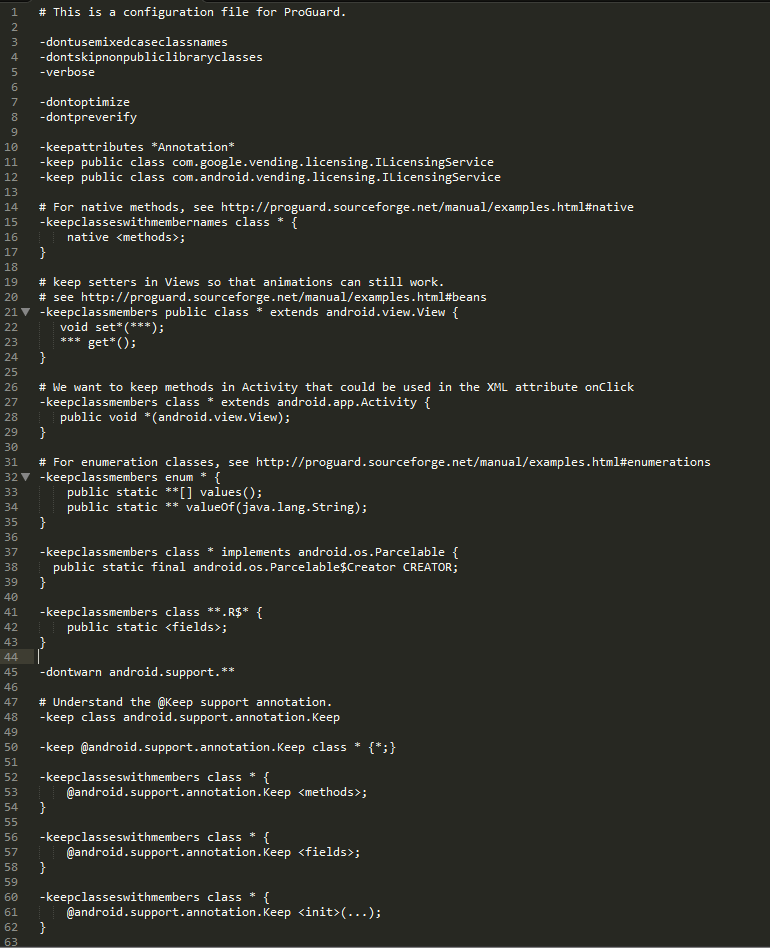
\includegraphics[width=1\textwidth]{figure/proguard-conf.png}
	\bicaption[fig:proguard-conf]{ProGuard Android配置样例}{ProGuard Android配置样例}{Fig}{Example of ProGuard Configuration for Android}
\end{figure}

图~\ref{fig:proguard-conf}为Android构建工具中使用的默认ProGuard配置。
而之前的混淆检测正是利用这份配置,可以看到在ProGuard默认配置中,只对资源类R的public static值域进行了保留,而在应用自身包内一定会存在R。
所以可以利用这一点来进行混淆检测,如果在应用对应包中没有发现R class,则将该应用认定为混淆应用。
这种快速简单的检测方式能够对绝大多数的混淆应用有效。

ProGuard的主要目标是让应用变得更小,同时使得应用的逆向工程变得更加困难。
表~\ref{tab:proguard-obs}展示了在ProGuard中用到的混淆技术,以及对应的配置设置。

\begin{table}[!hpb]
	\centering
	\bicaption[tab:proguard-obs]{ProGuard中不同混淆技术在Android构建中的配置开关}{ProGuard中不同混淆技术的配置开关}{Table}{ProGuard Configuration of 	Different Obfuscation Technique}
	\begin{tabularx}{\textwidth}{|X|c|c|c|X|X}
		\hline
		混淆技术 & 是否默认开启 & 配置开关 & 影响实体\\
		\hline
		标识符重命名 & \cmark & -dontobfuscate (关闭) & 包、类、方法\\
		\hline
		代码缩减 & \cmark & -dontshrink (关闭) & 包、类、方法\\
		\hline
		包结构平坦化 & \xmark & -flattenpackagehierarchy [package\_name] & 包\\
		\hline
		重打包类 & \xmark & -repackageclasses [package\_name] & 类\\
		\hline
		字节码优化 & \xmark & -dontoptimization & 类、方法\\
		\hline
	\end{tabularx}\\
\end{table}

在ProGuard中有两种包结构重组织的方法一种是包平坦化,一种是重打包类。
在进行包结构平坦化时,会将在混淆范围内的包重新组织到一个新的包中,包名为指定的package\_name,默认在根目录下;
而进行重打包类时,会将所有在混淆范围内的类重新打包到一个新包下,包名为指定的pacakge\_name,默认为根目录。
值得注意的是,包结构平坦化保留了一定程度的包结构信息,只是可能会去除掉子包的结构信息,而重打包类是完全去除了包的结构信息与子包的结构信息。

接下来,我们会根据上述总结的ProGuard规则设计我们相似度算法中指纹生成与指纹比对的方法。

\subsubsection{指纹生成}

在Java代码中,类是一个基础单元。
一个类包含着丰富的信息,包括所属包、父类、类的修饰符、成员变量、成员函数等等。
所以我们使用类为单元来进行指纹提取。
我们通过对类的稳定特性进行哈希来生成一个类的指纹。

而如何选择稳定特性是指纹生成的关键,也是相似度检测效果的关键。
由于混淆工具种类繁多,混淆技术花样百出,导致无法做到保证提取出的稳定特性在混淆前后保持不变。
并且即便存在不变的特性,这些特性包含的信息太少,造成太多的信息丢失,以至于在比对时会发生太多的误报,即原本不相似的两个类检测出相似度很高。
所以我们需要在其中找到权衡,在能保证在大多数混淆技术下能够稳定的前提下,要尽可能多的保留代码的信息,从而降低误报,使得相似度检测可用。

在本文所提出的方法中,我们使用的类的稳定特性包括三部分:成员函数,成员变量以及类的元信息。

\begin{itemize}
	\item \textbf{成员函数:} 一个成员函数由三部分组成,函数的修饰符、函数的签名以及函数的字节码。
		首先,函数的字节码在优化和混淆时会发生改变,例如死代码移除和随机化控制流等。
		并且由于混淆过程中会重命名标识符,所以稳定特性不能依赖于任何非Java核心类或者安卓框架类的类名和成员方法名,以及变量名。
		所以我们将这些易变的名字进行了一定程度的模糊处理,对于上述的名字,我们将会使用Object来代替。
		另外,当内联优化操作时,可能会将一个公共的getter内联,这可能就会把公共getter中使用到的私有变量更改成公共变量。
		在ProGuard中,如果allowaccessmodification和优化开启时,ProGuard会对代码进行内联优化,在此优化中,一个方法的access修饰符可能会被拓宽。
		因此我们应该将access修饰符从稳定特性中移除。
		综上所述,一个成员函数的稳定特性由模糊处理后的函数参数类型,函数返回类型,以及部分函数修饰符构成。
	\item \textbf{成员变量:} 一个成员变量由三部分组成,变量的修饰符、变量的类型以及变量的名字。
		由于标识符重命名以及内联优化,我们不能依赖于变量的名字以及access修饰符。
		所以成员变量的稳定特性由模糊处理后的变量类型和部分变量修饰符组成。
	\item \textbf{类元信息:}除了成员函数与变量之外,还有一些额外的信息可以选进类的稳定特性。
		当声明一个类,需要声明类的修饰符、类的父类以及实现的接口。
		在ProGuard中,如果allowaccessmodification和repacakgeclasses开启时,混淆器会将所有重命名过的类重新打包到一个特定的包中。
		因此被重新打包的类的access修饰符可能在重打包过程中被修改。
		因此类的access修饰符不应该被包含在类的稳定特性中。
		最终一个类元信息的稳定特性由模糊处理后的父类类型以及模糊处理后的实现的接口类型。
\end{itemize}

在提取出一个类的所有稳定特性之后,我们需要生成这个类的指纹信息。
我们通过对以上稳定特性分别哈希,得出三个哈希值的列表,分别为成员函数的稳定特性哈希值列表、成员变量的稳定特性哈希值列表以及类元信息的稳定特性哈希值列表。

\subsection{指纹比对}

在比对过程中,有些研究的做法是将类的所有模糊处理后的成员函数签名排序后进行哈希,最后通过比对两个类的哈希值是否相同来判断两个类是否一样。
由于代码缩减的存在,一个类在经过混淆之后,未使用过的成员方法或者成员变量可能会被剔除。
所以一个类在混淆前后的指纹是会发生改变的,其中元信息指纹不会改变,成员变量和成员函数的指纹列表可能会有所缩减。
因此上述方法在处理混淆应用时可能存在问题,导致漏报率增加。

一对同源类A和B存在三种关系:

\begin{enumerate}
	\item A为初始类,经过混淆后变成了B。此时A的成员变量和成员函数指纹列表是B的超集;
	\item A为初始类,经过混淆后变成了B。此时A的成员变量和成员函数指纹列表是B的超集;
	\item A,B都为未混淆类C混淆处理后的类。此时A和B的成员变量和成员	函数指纹信息列表会有相同的指纹元素,也会因为剔除的方法和变量不同而产生差异。
\end{enumerate}

在比对算法中,我们使用了严格相似的标准,即只有出现了上述情况中的前两种我们才会标记类B相似于类A或者类A相似于类B。
在实现中,对于两个类A和B:

\begin{enumerate}
	\item 判断A和B的元信息指纹是否相同;
	\item 判断成员变量指纹列表和成员函数指纹列表是否存在包含关系,如果A包含B,那么标记B相似于A,反之则标记B相似于A,如果A与B一样,则同时标记A相似于B以及B相似于A。
\end{enumerate}

% 由于同构的类经常出现,例如属于Android v4 support library(相同包)的\texttt{SlidingPaneLayout\$SavedState\$1}和\texttt{DrawerLayout\$SavedState\$1},以及Android v4 support library 的\texttt{SlidingPaneLayout\$SavedState\$1}和Android v7 support library的\texttt{Toolbar\$SavedState\$1}(不同包)。
另外,由于代码缩减技术的存在,很多本身不同构的类去除掉没有用掉的成员变量和函数之后,可能会形成同构的情况。
同构类导致类的指纹不是唯一的,所以两个应用的相同指纹的类多并不能代表这两个应用相似。
在这种情况下,就需要引入包的信息来减少同构类造成的误报。

Java中,包的作用是组织类,一个包中包含一组类或接口,这些类和接口功能相关,所以组织在一个包中方便类的查找和使用。
另外包也决定了类的命名空间,包采用树形的存储方式,在一个包中的类的名字不能相同,但是在不同包中的类,名字可以相同。
同时包也规定了包中类的访问权限,以便于更稳定的组织。

由于是文件夹的组织形式,一个包可能包含子包,即子包在母包文件夹下。
这种包之间的关系可能会由于混淆中的包结构重组织而改变,有可能混淆前B是A的子包,而在混淆后B可能已经存在于另外一个包中了。
所以在我们的指纹比对算法中,不会考虑包之间的包含关系。


最后对于一对包A和B,我们会计算出两个相似度\emph{Sim$_{AB}$}和\emph{Sim$_{BA}$}:
\begin{equation}
	\emph{Sim$_{AB}$} = \frac{|\emph{Class$_{AB}$}|}{|\emph{Class$_{A}$}|}.
\end{equation}

\begin{equation}
	\emph{Sim$_{AB}$} = \frac{|\emph{Class$_{AB}$}|}{|\emph{Class$_{A}$}|}.
\end{equation}

其中\emph{Class$_{BA}$}为包B中与包A中相似的类的集合,\emph{Class$_{AB}$}为包A中与包B中相似的类的集合。
而\emph{Class$_{A}$}和\emph{Class$_{B}$}分别表示A和B中类的集合。
当\emph{Sim$_{AB}$}或者\emph{Sim$_{BA}$}超过设置的阈值时,我们会判断A相似于B或者B相似于A。

\subsection{第三方库检测}

AppShield中的第三方库检测基于上文所介绍的相似度检测方法。
我们会收集需要检测的第三方库的不同版本SDK,并对其进行指纹提取。
在实现上,我们先将第三方库的SDK jar包使用Android构建工具dx打包成APK,之后就能使用之前提到的相似度检测的方法。
我们将要检测的应用的指纹与所有版本的SDK指纹一一比对,比如对于一个应用A和n个版本的第三方库B$_{1}$ - B$_{n}$,如果发现任意一个版本的B$_{i}$,\emph{Sim$_{B_{i}A}$}超过了0.7,那么我们就判断应用A包含第三方库B。

\subsection{克隆应用检测}

AppShield中的克隆应用检测同样也是基于相似度检测的方法。
由于在克隆应用中,只会重打包很少一部分信息,所以互相的相似度都应该要求在一个很高的水平上,并不会出现克隆应用A和B,A相似与B而B不相似于A。
所以在实现上我们将相似度比对的阈值设置在了0.9,并且需要\emph{Sim$_{AB}$}和\emph{Sim$_{BA}$}同时超过了阈值,我们才将这对应用标记为潜在的克隆应用。

\section{本章小结}
\label{sec:appshield:conclusion}

本章对AppShield的设计与实现做了详细的介绍。
首先介绍了AppShield大致架构,其次对应用文件来源进行了阐述,之后对问题组件分析模块进行了描述,最后对AppShield中第三方库检测和克隆应用检测用到的相似度分析方法进行了介绍。
\chapter{测试与评估}
\label{chap:evaluation}

在本章中,我们将对第四章介绍的AppShield系统进行测试与评估,这主要包括隐私问题检测与相似度检测部分。
在~\ref{sec:test-set}节中,我们简单介绍了经过两年时间收集的测试集;
在~\ref{sec:privacy-eval}节中我们对AppShield检测隐私问题的能力进行测试与评估,并挑选了被发现隐私问题样本数较高的广告库Tapjoy,进行了详细的案例分析;
在~\ref{sec:sim-eval}节中我们对AppShield使用的相似度检测方法进行了测试与评估。
最后在~\ref{sec:eval:conclusion}节中我们将对本章进行小结。

\section{测试集}
\label{sec:test-set}


AppShield系统的测试数据集主要来自于AppShield的爬虫程序,同时也包括一些已知的恶意软件库。
总计分析应用数量超过14万,应用文件数据量已经超过4.5TB磁盘空间,分析结果数据库约为45GB,表~\ref{tab:test-set}为测试集的基本情况。

\begin{table}
	\centering
	\bicaption[tab:test-set]{AppShield测试集}{AppShield测试集}{Table}{Test Set of AppShield}
	\begin{tabularx}{\textwidth}{|X|c|X|X|}
		\hline
		市场名字 & 应用数量 & 市场类型 & 链接\\
		\hline
		Google Play & 116672 & 北美、欧洲官方应用市场 & \url{https://play.google.com/store/apps}\\
		\hline
		Android Drawer & 6537 & 北美第三方市场 & \url{http://www.androiddrawer.com/}\\
		\hline
		酷安网 & 8171 & 国内第三方市场 & \url{http://www.coolapk.com/}\\
		\hline
		腾讯应用宝 & 10993 & 国内第三方市场 & \url{http://www.myapp.com/}\\
		\hline
		机锋网 & 1913 & 国内第三方市场 & \url{http://apk.gfan.com}\\
		\hline
		Android病毒基因库 & 1260 & 已知恶意应用库 & \url{http://www.malgenomeproject.org/}\\
		\hline
		美国North Eastern大学研究数据库 & 1278 + 3063 & 普通应用以及恶意样本 & 帮助美国科研团队评估科研成果有效性,\url{http://recon.meddle.mobi/}\\
		\hline
		用户上传 & 1366 & 任意 & 通过 \newline 
								\url{http://appaudit.io}\\
		\hline
	\end{tabularx}
\end{table}


我们的测试集具有以下特点:

\begin{enumerate}
	\item 涵盖官方与非官方的应用市场。
	\item 涵盖国内与国外的应用市场。
	\item 涵盖移动量的已知恶意应用,可以评估AppShield的有效性
\end{enumerate}

搜集的市场元数据包括:应用上传时间、大小、更新时间、Google Play评分、开发者名字、开发者联系方式、市场内相关应用、下载量、一些评论、分类tag、45款主流杀毒软件病毒检测结果、图标、展示图片、展示视频、内容分级、隐私报告等等。这些信息帮助我们对检测到的隐私问题的应用进行影响因子排序。

\section{隐私问题检测}
\label{sec:privacy-eval}

在AppShield中使用了AppAudit进行单应用审查。
其中AppAudit在基准病毒样本库Android Malware Genome Project上的测试准确度可以达到99.3\%,在检测时间上AppAudit可以在平均几秒钟的时间内完成一个应用的审查,并且审查一个应用的内存使用量只需要200MB以内,普遍优于现有学术研究以及Google应用市场的产品,对于AppAudit详细的测试评估可以参考AppAudit的论文。

对于应用市场内的隐私泄露情况,AppShield会总结出泄露应用列表以及泄露概要,来对市场内的隐私泄露情况进行评估与分析。

\subsection{隐私泄露情况总览}

在检测到的隐私泄露中,有些位于第三方库组件中,有些位于应用开发者自己开发的组件中。
我们将AppShield分析收集到的泄露信息进行汇总,并将属于应用本身的组件归纳为一类,记做“app\_itself”。
图~\ref{fig:leak-comp}为汇总之后,组件被检测出泄露信息频次最多的20个组件。

\begin{figure}
	\centering
	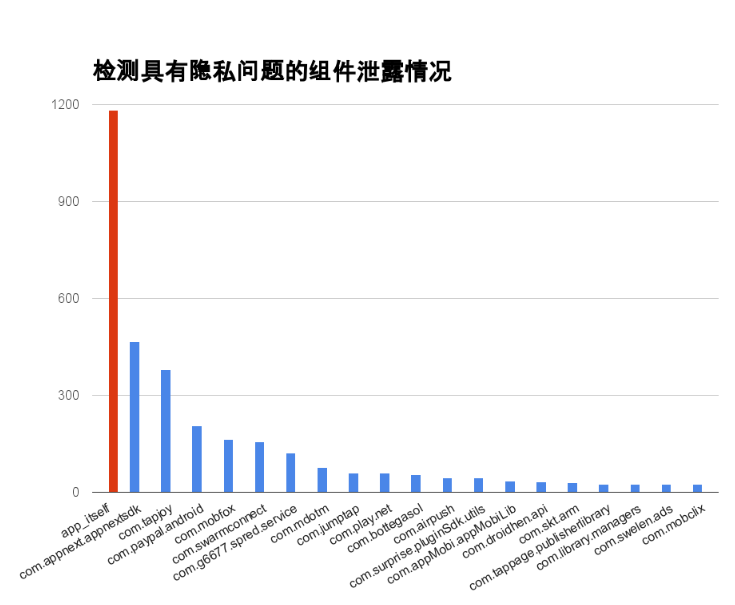
\includegraphics[width=1\textwidth]{figure/leak-comp.png}
	\bicaption[fig:leak-comp]{具有隐私问题的组件泄露情况}{具有隐私问题的组件泄露情况}{Fig}{Leakage Information of Problematic Components}
\end{figure}

从图中可以看出,应用本身的隐私泄露情况是最普遍的,大约占据3成左右,剩下的7成都是第三方组件库导致的隐私泄露问题。
前20个隐私泄露频次最多的组件中,第三方广告库就占有着很大的比例,其中Tapjoy、Mobfox都是流行度比较高的广告库,在Appbrain对官方Google Play市场的份额统计中,已安装应用分别有5.66\%、0.73\%的应用使用了这两家广告库(达到5.66万个以及7300个应用使用这些有问题的库)。
由于广告库是这次分析隐私泄露的重灾区,我们会在之后的问题部件案例分析中着重介绍。

\begin{figure}
	\centering
	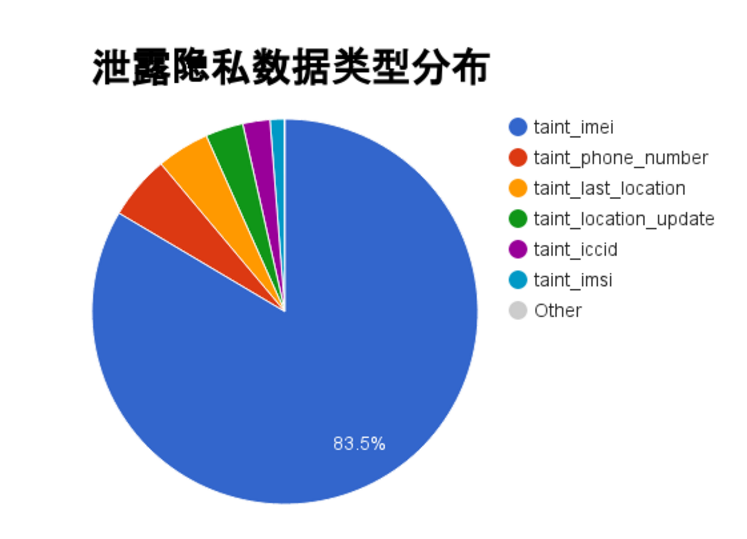
\includegraphics[width=0.7\textwidth]{figure/leak-type.png}
	\bicaption[fig:leak-type]{泄露隐私数据类型分布}{泄露隐私数据类型分布}{Fig}{Distribution of Leakage Information Type}
\end{figure}

我们以泄露的信息为关注点,图~\ref{fig:leak-type}为在所有组件中泄露隐私信息类型的情况分布图。

可以看出泄露情况最严重的是IMEI,即国际移动设备标识,占总泄露频次的83.5\%。
IMEI是手机的唯一识别号码,由15位数字组成,前6位数是“型号核准号码”(TAC,Type Approval Code),代表机型。接着的2位数为“最后装配号”(FAC,Final Assembly Code),代表产地。之后的6位数是“串号”(SNR,Serial Number),代表生产顺序号。最后1位数通常是“0”,为检验码。

IMEI本身包含的隐私信息有限,但是IMEI经常被应用用来当作识别一个手机的标识。
所以如果IMEI被泄露,可能会存在潜在的安全隐患。
WhatsApp在三年前被曝光使用手机的号码当作用户名,使用IMEI的md5值作为密码。
在这种情况下,IMEI被泄露就相当于WhatsApp的密码被泄露,是一个严重的安全隐患。

除开IMEI之外,其他的隐私信息的泄露情况也是不可忽视的。
相比IMEI,电话号码以及地理位置相关的隐私信息被泄露带来的安全隐患可能大得多,所以应用的隐私泄露是一个需要被应用市场关注的领域。

\subsection{问题组件分析}

针对泄露隐私问题最严重的广告类库,我们挑选了检测出泄露情况较多的几个广告库进行了作为样例进行数据汇总以及可视化。
根据AppShield的问题组件分析,找出对应广告库的不同版本,并获取应用不同版本广告库的引用的单应用审查结果,最终得出统计结果。
并且,我们着重对Tapjoy进行了详细的案例分析。

\begin{table}
	\centering
	\bicaption[tab:adlib-overview]{广告库相关基本信息}{广告库相关基本信息}{Table}{General Information of Related Advertise Libraries}
	\begin{tabularx}{\textwidth}{|c|c|c|X|}
		\hline
		广告库 & 地区 & 成立时间 & 特点\\
		\hline
		Tapjoy & 北美 & 2007 & 活跃用户高 覆盖面广\\
		\hline
		Mdotm & 北美 & 2009 & 基于表现的广告投放 跨渠道\\
		\hline
		MobFox & 欧洲 & 2010 & 针对欧洲 提供广告服务端和应用优化服务\\
		\hline
	\end{tabularx}
\end{table}

\begin{table}
	\centering
	\bicaption[tab:adlib-leak]{广告库在AppShield中的分析结果统计数据}{广告库在AppShield中的分析结果统计数据}{Table}{Analysis Statistics of AppShield for Advertise Library}
	\begin{tabular}{|c|c|c|c|c|}
		\hline
		广告库 & 泄露样本数 & 总样本数 & 泄露版本数 & 总版本数\\
		\hline
		Tapjoy & 379 & 3447 & 31 & 103\\
		\hline
		Mdotm & 77 & 92 & 2 & 2\\
		\hline
		MobFox & 163 & 178 & 12 & 12\\
		\hline
	\end{tabular}
\end{table}


我们一共挑选了三个广告库样例,分别为Tapjoy,MdotM(已更名为CrossChannel)以及MobFox。
表~\ref{tab:adlib-overview}介绍了三个广告库的基本信息以及特点。

在AppShield深度问题组件分析中,Tapjoy组件被识别一共有103个版本,其中31个版本被AppAudit检测出有隐私泄露行为;
MobFox的版本总量相对Tapjoy少了很多,仅有12个版本,并且12个版本均被AppShield检测出有隐私泄露行为;
而MdotM(CrossChannel)仅被检测出在测试集中有2个样本,并且2个样本均有泄露隐私行为。
图~\ref{fig:leak}为不同广告库版本在测试集中的使用情况,其中红色的表明被检测出隐私泄露的数量。
表~\ref{tab:adlib-leak}为这三个广告库在AppShield中检测的相关数据。

\begin{figure}
  \centering
  \subfigure[Tapjoy]{
    \label{fig:leak:tapjoy} %% label for first subfigure
    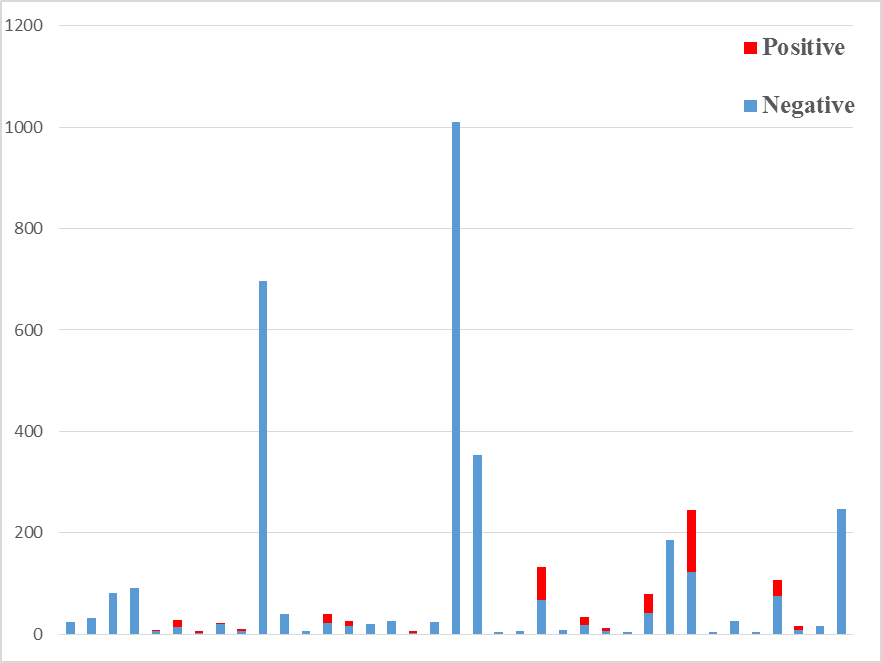
\includegraphics[width=1\textwidth]{figure/tapjoy-leak.png}
  }

  \subfigure[MobFox]{
    \label{fig:leak:mobfox} %% label for second subfigure
    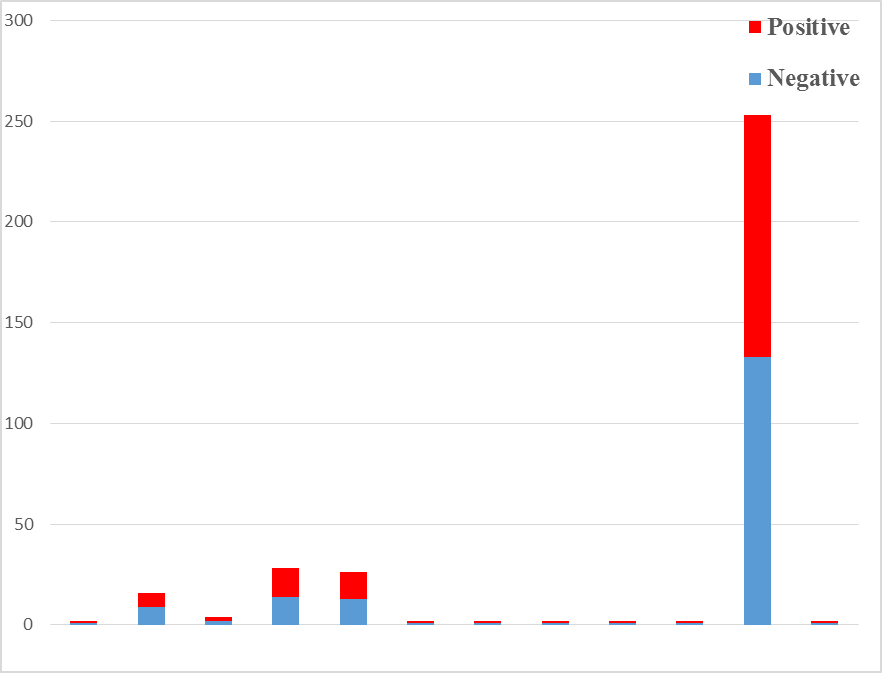
\includegraphics[width=0.4\textwidth]{figure/mobfox-leak.png}
  }
  \subfigure[Mdotm]{
  	\label{fig:leak:mdotm}
  	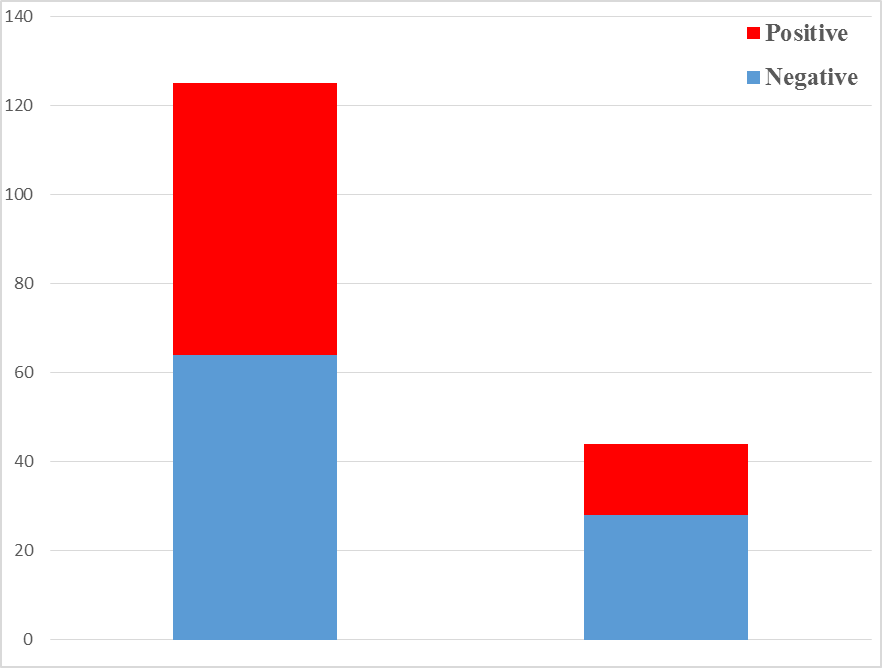
\includegraphics[width=0.4\textwidth]{figure/mdotm-leak.png}
  }
  \bicaption[fig:leak]{不同版本广告库泄露隐私情况}{不同版本广告库泄露隐私情况}{Fig}{Sensitive Information Leak among Different Versions of Ad Lib SDK}
\end{figure}

Tapjoy是一家美国的移动广告平台,成立于2007年,目前覆盖了10亿台全球移动设备,全球月活跃用户高达5.05亿。
应用开发者能利用Tapjoy的SDK,在应用中插入Tapjoy提供的广告,因而来将应用的流量变现。

在AppShield的分析中检测出Tapjoy组件会在应用运行的过程中会泄露手机的IMEI信息,我们接着对出现问题的应用进行反编译,确认了泄露的路径,并整理出了Tapjoy在工作过程中会收集并且通过HTTP传输出去的信息。
表~\ref{tab:tapjoy-leak}为我们分析得出的Tapjoy SDK会收集的用户信息列表,我们对敏感数据进行了标红处理。

\begin{table}
	\centering
	\bicaption[tab:tapjoy-leak]{Tapjoy SDK收集的用户信息}{Tapjoy SDK收集的用户信息}{Table}{User Information List of Tapjoy SDK will Collect}
	\begin{tabularx}{\textwidth}{|l|X|}
		\hline
		参数名 & 描述\\
		\hline
		app\_id & Tapjoy开发者对应的app\_id\\
		\hline
		android\_id & 用户第一次打开设备时随机生成的一个64位的数字字符串,当用户恢复出厂设置时,这个值会重新随机生成\\
		\hline
		{\color{red}udid} & IMEI\\
		\hline
		sha2\_udid & IMEI的SHA-256\\
		\hline
		sha1\_mac\_address & 设备mac地址的SHA-1\\
		\hline
		serial & 硬件的串号\\
		\hline
		device\_name & 终端用户的设备名称\\
		\hline
		device\_manufacturer & 设备的制造商\\
		\hline
		os\_version & 操作系统版本\\
		\hline
		country\_code & 国家代码\\
		\hline
		language\_code & 语言代码\\
		\hline
		{\color{red}package\_names} & 设备当前安装的应用列表\\
		\hline
	\end{tabularx}
\end{table}


之前讨论了泄露IMEI的危害,在Tapjoy SDK中,还会尝试去获得设备当前安装的应用列表,这其实也是一个比较敏感的信息。
之前有案例是通过手机病毒获取受害者手机上安装的应用列表,从而得知用户手机中是否安装了银行类的应用,利用这个信息使用社会工程学进行诈骗。

\begin{figure}
	\centering
	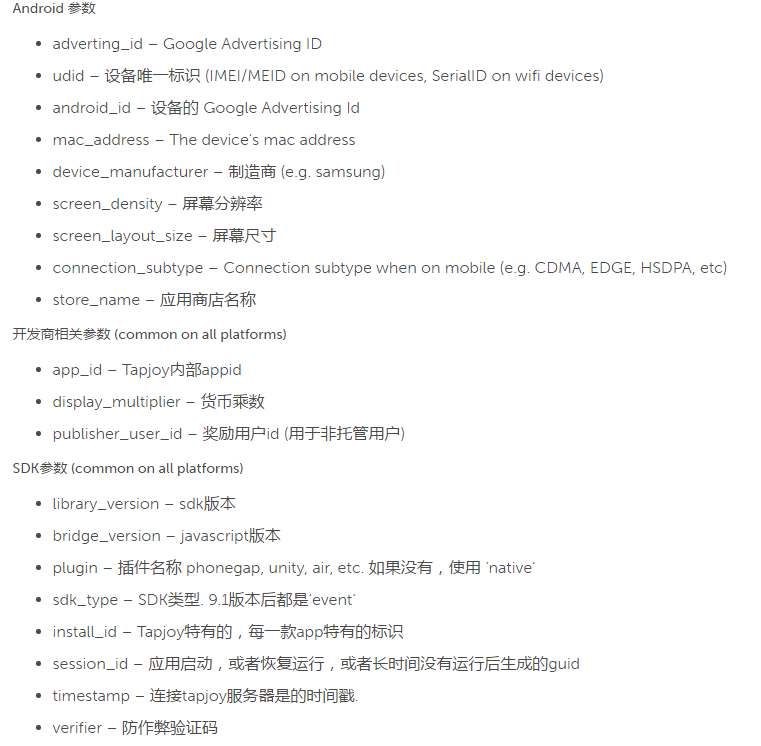
\includegraphics[width=0.6\textwidth]{figure/privacy-policy.png}
	\bicaption[fig:privacy-policy]{Tapjoy官方网站隐私声明}{Tapjoy官方网站隐私声明}{Fig}{Privacy Policy of Tapjoy}
\end{figure}

图~\ref{fig:privacy-policy}展示了Tapjoy在官网中声明的Tapjoy SDK会收集的信息。
Tapjoy声称会将手机到的用户信息安全保护好,不允许未授权机构或个人访问。
另外Tapjoy会将用户信息与合作伙伴、Tapjoy相关分支机构以及广告商等共享,从而给用户提供更好的广告服务。

从图~\ref{fig:leak:tapjoy}可以看出,Tapjoy SDK更新比较活跃,有隐私泄露行为的版本只占了总版本数的一小部分。
并且在最新的SDK版本中(v10.2.2),Tapjoy也添加了将IMEI进行SHA-256的代码,只使用IMEI哈希之后的值。
这样就能将隐私信息进行匿名化,同时能同样标识用户的设备。
图~\ref{fig:tapjoy-code}为Tapjoy SDK对IMEI进行SHA-256匿名化的代码片段。

\begin{figure}[!h]
	\centering
	\begin{lstlisting}[language={java}]
	if (isPermissionGranted("android.permission.READ_PHONE_STATE")) {
		try {
			if (getConnectFlagValue(TapjoyConnectFlag.DEBUG_DEVICE_ID) == null || getConnectFlagValue(TapjoyConnectFlag.DEBUG_DEVICE_ID).length() <= 0) {
				deviceID = telephonyManager.getDeviceId();
			} else {
				deviceiD = getConnectFlagValue(TapjoyConnectFlag.DEBUG_DEVICE_ID);
			}
			TapjoyLog.i(TAG, "deviceID: " + deviceID);
			...
			if (validDeviceID) {
				sha2DeviceID = TapjoyUtil.SHA256(deviceID);
				return;
			}
			...
		}
	}
	\end{lstlisting}
	\bicaption[fig:tapjoy-code]{最新版本Tapjoy SDK中对IMEI进行了SHA-256操作的相关代码}{最新版本Tapjoy SDK v10.2.2中对IMEI进行了SHA-256操作的相关代码}{Fig}{Code Snippet of Tapjoy SDK v10.2.2}
\end{figure}



另外在进行案例分析中,我们发现MobFox和Mdotm组件的所有版本都有被检测出泄露隐私信息行为的样本,但是仍有一小部分同版本的样本没有被AppAudit检测出有安全隐患。

从图~\ref{fig:leak:mobfox}中可以看到,MobFox第二条直方一共存在130多个应用使用了同一个Mobfox SDK版本。
然而在这130多个应用中有将近120个被AppAudit识别出存在隐私问题,由此可以推断未被标记的10多个应用很可能就是AppAudit存在遗漏的有隐私问题的样本。
这些样本可以帮助AppAudit开发者快速找到遗漏样本并对工具本身进行修正。
同样的如果途中某个版本大量样本没有问题,只有少数被标记,则可以推断这些被标记的样本可能是单应用审查工具的误报案例,同样可以帮助这类工具。
在AppShield中由于AppAudit设计中不会出现误报,只有遗漏,所以相应的在AppShield的分析中只会出现某个版本的样本中疑似有遗漏。

\section{相似度检测}
\label{sec:sim-eval}

我们还对提出的相似度检测的方法进行了测试评估。
我们首先对相似度检测方法处理混淆能力、检测时间进行了测试。
之后我们挑选了10种第三方库以及他们的不同版本,一共53个SDK,来对我们测试集中10993个来自腾讯应用宝市场上的应用进行了第三方库检测,来检验我们的相似度检测方法是否在给出问题组件的前提下,找出包含问题组件的应用。
最后我们还挑选了1000个应用,对其进行了重打包应用的检测。

\subsection{微基准测试}

在微基准测试中,我们人工编写了集成了多个第三方库的应用,并使用此应用的未混淆版本以及经过了不同配置后的混淆处理之后的应用进行相似度检测,从而检验本文的相似度检测方法是否有能力处理混淆。

我们编写的应用一共集成了4个第三方库,处理JSON的工具库gson,提供类型安全的HTTP客户端retrofit,另外还有retrofit依赖的两个库okhttp和okio。

由于代码缩减的检测依赖于应用对第三方库的使用情况,所以我们在应用中对几个第三方库进行了基本功能的使用,从而模拟真实应用的情况。我们的对照组为未混淆过的应用,实验组有6个。

\begin{table}
	\centering
	\bicaption[tab:micro-bench]{相似度检测微基准测试结果}{相似度检测微基准测试结果}{Table}{Micro-benchmark Result of Similarity Detection}
	\begin{tabular}{|c|c|c|c|c|c|c|}
		\hline
		 & 标识符重命名 & 平铺化包 & 重打包类 & 代码缩减 & 代码优化 & 相似度\\
		\hline
		试验组1 & 1 & 0 & 0 & 0 & 0 & 1\\
		\hline
		试验组2 & 0 & 1 & 0 & 0 & 0 & 1\\
		\hline
		试验组3 & 0 & 0 & 1 & 0 & 0 & 0.21\\
		\hline
		试验组4 & 0 & 0 & 0 & 1 & 0 & 0.63\\
		\hline
		试验组5 & 0 & 0 & 0 & 0 & 1 & 0.8\\
		\hline
		试验组6 & 1 & 1 & 0 & 1 & 0 & 0.75\\
		\hline
	\end{tabular}
\end{table}


实验结果如表~\ref{tab:micro-bench}所示,可以看出我们的相似度检测方法可以很好的应对标识符重命名、代码缩减以及代码优化,能在一定程度上处理包平铺化,对重打包类处理能力较差。
主要是因为我们利用了包的层次信息,包平铺化只会在一定程度上保留包层次信息,而重打包类完全破坏了此信息。

但是在实验中我们也发现了重打包类混淆技术的一些特点。
由于重打包类会将所有混淆的类重新打包到一个新的包中,所以当我们发现一个包中的类匹配了来自很多不同包内的类时,可能此包为重打包混淆中的新包。
以此发现为基准,可能可以发明一些启发式的算法,来发现应用是否经过了重打包混淆,并尝试进行识别。

在指纹生成阶段,一共包括4个步骤:
\begin{enumerate}
	\item 解压缩apk包
	\item 使用baksmali将dex代码反编译成smali代码
	\item 解析smali代码,将其结构化以便生成指纹
	\item 对稳定特性进行SHA1指纹生成
\end{enumerate}

图~\ref{fig:fingerprint-time}展示了10993个应用在指纹生成过程中每一步所花费的时间,可以看出SHA1生成指纹这一步明显随着类的数量增加而提升,而其余几步随着类的增加基本趋于稳定。

\begin{figure}
	\centering
	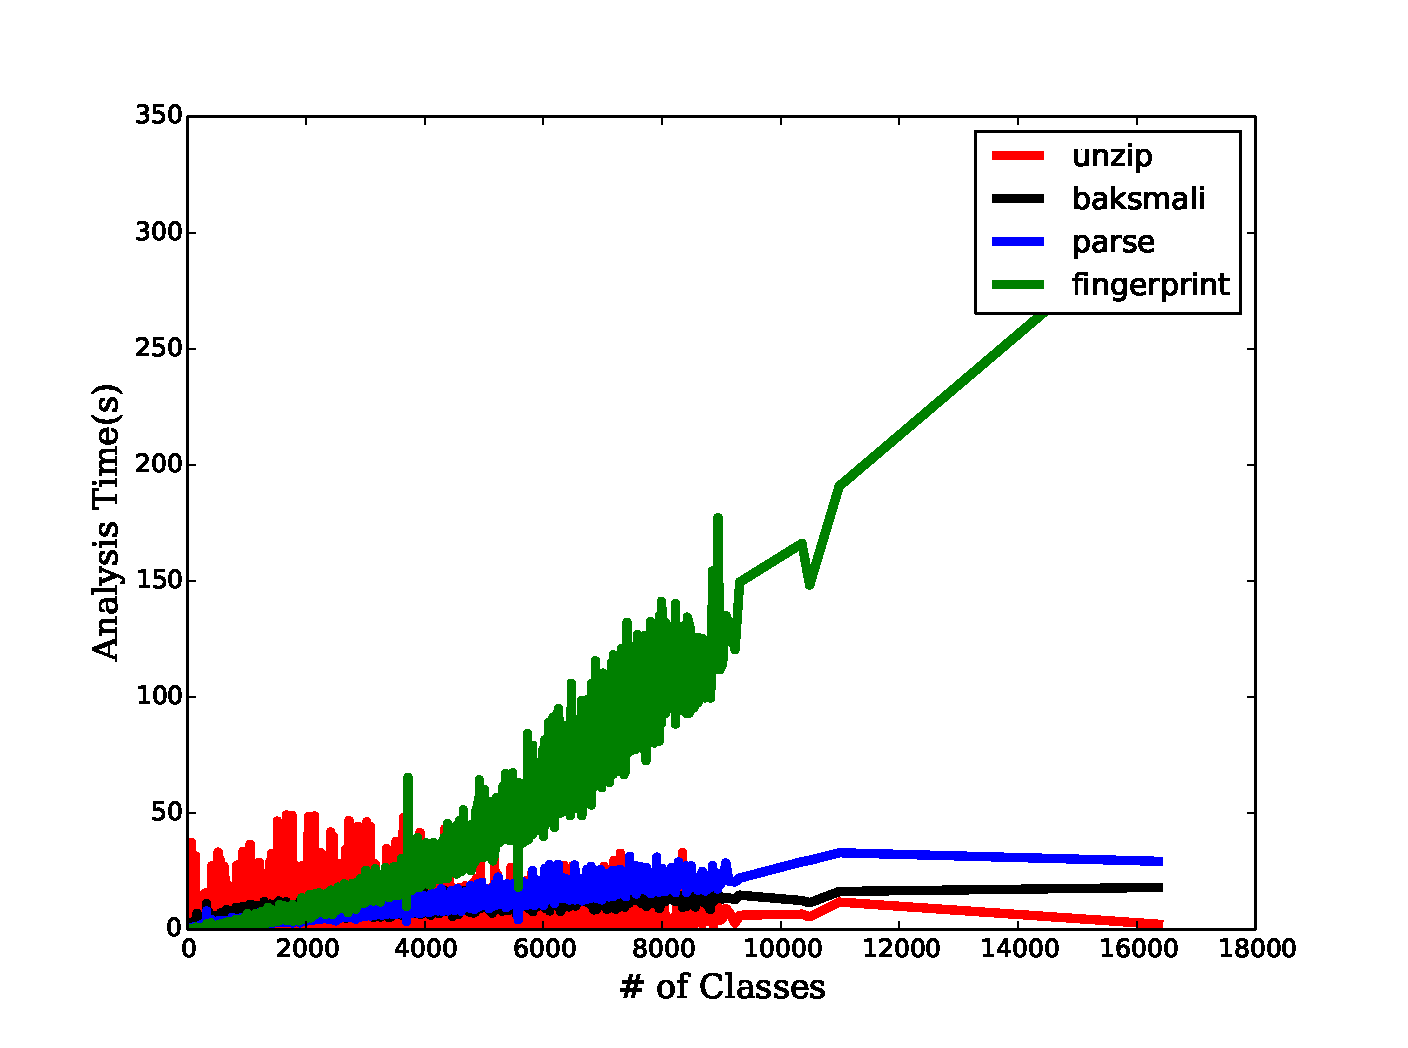
\includegraphics[width=0.8\textwidth]{figure/time-cdf.eps}
	\bicaption[fig:fingerprint-time]{指纹生成各部分时间CDF图}{指纹生成各部分时间CDF图}{Fig}{CDF of Different Part of Time in Fingerprint Generate}
\end{figure}

\subsection{第三方库检测}

在第三方库检测的实验中,我们人工获取了6个第三方库的67个SDK版本。
表~\ref{tab:sdk-overview}为这些SDK的基本信息。

\begin{table}
	\centering
	\bicaption[tab:sdk-overview]{SDK相关信息}{SDK相关信息}{Table}{Information of Selected SDK}
	\begin{tabularx}{\textwidth}{|X|X|X|c|}
		\hline
		SDK名 & 包名 & 功能 & 版本数\\
		\hline
		gson & \texttt{com.google.gson} & 提供JSON相关操作 & 20\\
		\hline
		okhttp & \texttt{com.squareup.okhttp3} & HTTP客户端 & 12\\
		\hline
		retrofit & \texttt{com.squareup.retrofit}\newline\texttt{com.squareup.retrofit2} & 类型安全的HTTP客户端 & 15\\
		\hline
		weibo核心SDK & \texttt{com.sina.weibo}\newline\texttt{com.sina.sso} & 提供微博接入相关功能 & 6\\
		\hline
		友盟SDK & \texttt{com.umeng.analytics} & 提供应用统计相关功能 & 13\\
		\hline
		Talking Data SDK & \texttt{com.tendcloud.tenddata} & 提供应用统计相关功能 & 1\\
		\hline
	\end{tabularx}
\end{table}

10993个应用的检测结果如表~\ref{tab:third-detect}所示,在使用的这来自6个第三方库的67个SDK版本检测中,至少被检测出含有一个第三方库的应用有1803个,占全部的16.4\%。
其中gson检测率最高,被1230个应用使用,占全部的10.26\%。

\begin{table}
	\centering
	\bicaption[tab:third-detect]{第三方库检测结果}{第三方库检测结果}{Table}{Analysis Result of Third-Party Library Detection}
	\begin{tabular}{|c|c|c|}
		\hline
		SDK & 应用数 & 比例\\
		\hline
		gson & 1230 & 10.26\%\\
		\hline
		友盟SDK & 748 & 6.24\$\\
		\hline
		Weibo核心SDK & 282 & 2.35\%\\
		\hline
		okhttp & 85 & 0.71\%\\
		\hline
		retrofit & 58 & 0.48\%\\
		\hline
		Talking Data SDK & 15 & 0.13\%\\
		\hline
	\end{tabular}
\end{table}


本实验为原型实验,证明了第三方库检测的可行性。
之后可以通过持续从maven数据库获取第三方库的SDK来建立完备的第三方库数据库,对应用实现更全面准确的检测。

\subsection{克隆应用检测}

在检测结果中有很多只含有一个包的应用,并且这些应用之间的相似度都为1。
我们人工分析了这些“特殊”的应用,发现这些应用是通过了奇虎360加固保处理后的应用,这些应用一共有1270个。
360加固保使用通常我们说的应用“加壳”的方式对应用进行保护,通过重打包,对应用代码进行加密、运行时完整性检验等方式防止应用被篡改以及被分析。
我们将结果中所有使用了奇虎360加固保处理的应用结果剔除,来防止其对测试集造成的影响。

我们一共挑选了1000个应用进行克隆应用的检测,一共存在499500个比对结果。
图~\ref{fig:sim-cdf}为应用相似度的CDF图。

\begin{figure}
	\centering
	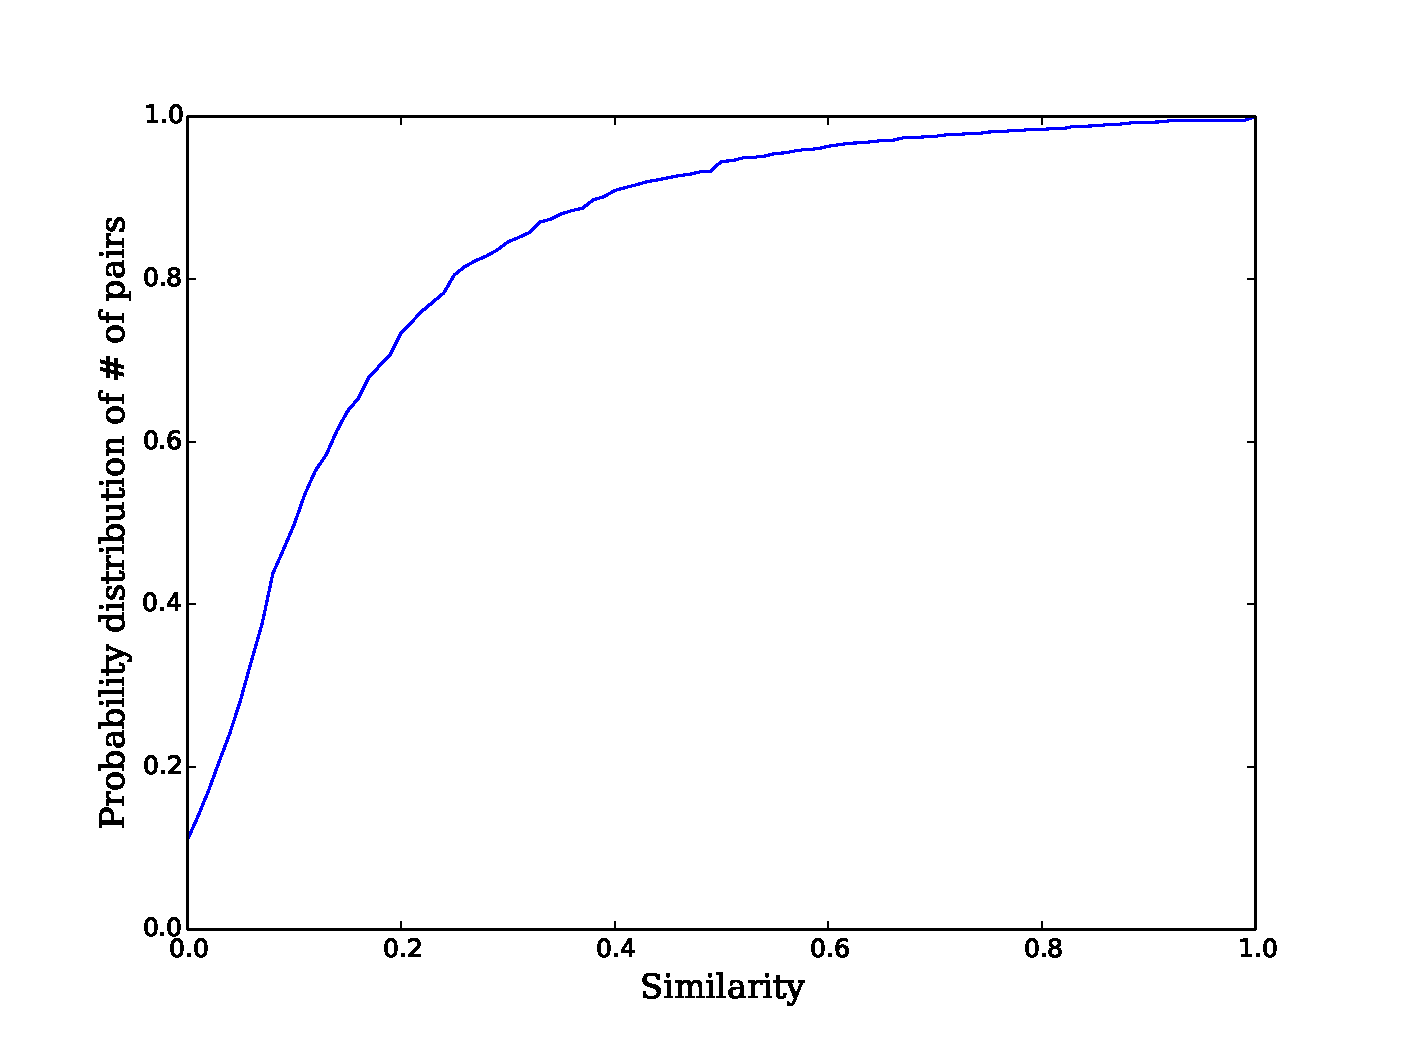
\includegraphics[width=0.6\textwidth]{figure/sim-cdf.eps}
	\bicaption[fig:sim-cdf]{应用相似度CDF图}{应用相似度CDF图}{Fig}{CDF of Similarity between Applications}
\end{figure}

从图中可知,高于在克隆应用检测阶段设置的相似度阈值0.9的有0.7\%的应用。

在我们检测出的潜在克隆应用对中,我们人工确认了一例开发者以不同应用名将同一应用上传应用市场多次的事例。
图~\ref{fig:clone-app}为这一对应用,这一对应用的相似度为1,开发者密钥相同,但有着不同的包名以及应用名。
这说明着,在中国市场上的确存在开发者仅修改应用名和包名,就将同一应用多次上传至应用市场,来提高应用的曝光的可能性。

\begin{figure}
	\centering
	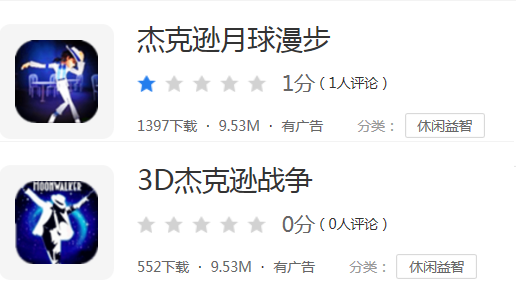
\includegraphics[width=0.6\textwidth]{figure/clone-pair.png}
	\bicaption[fig:clone-app]{不同应用名的相同应用}{不同应用名的相同应用}{Fig}{Same Application of Different Application Names in Myapp}
\end{figure}

可以看出,我们的克隆应用检测误报率很高。
在经过对误报样本进行人工确认之后发现,很多相似度很高的应用只是因为使用了相同的第三方库,而应用本身逻辑在应用所有代码中占比很小。
所以如果需要提高检测的准确性,需要剔除掉应用使用的第三方库,找出应用真正的逻辑,进行比对。

\section{本章小结}
\label{sec:eval:conclusion}

在本章中,我们对AppShield的隐私问题分析以及相似度检测两方面进行了测试与评估。
测试集一共包含13万多的应用,来自国内外各大应用市场。
首先我们对AppShield的隐私问题分析部分进行了测试。
在测试集中,我们成功分析了14万样本,找到超过9000多例的隐私泄露应用,并总结出超过20个有隐私问题的问题部件,并对隐私泄露方式进行了总结与可视化。
然后我们对AppShield的相似度检测部分进行了测试评估。
我们选取了来自腾讯应用宝市场的10993个应用进行了第三方库的检测,对8个第三方库的67个SDK版本进行检测,最终检测出超过10\%的应用包含gson库,超过6\%的应用包含友盟SDK。
结果验证了相似度检测的方法能够较好的应用与第三方库的检测中。
最后我们挑选了1000个应用进行克隆应用检测,最终检测出一例开发者以不同应用名将应用重复上传至应用市场的事例。
\chapter{总结与展望}
\label{chap:conclusion}

本章对全文进行总结与展望,主要包括对本文所做贡献进行总结,分析系统中现有的不足之处,对可改进之处进行展望。

\section{总结}

随着移动互联网的爆炸式发展,移动应用的使用越来越频繁,而移动应用的数量也在成几何增长。
然而移动应用的质量参差不齐,其中也不乏有很多盗取用户隐私恶意应用和克隆应用。
为了解决这个问题,我们设计了AppShield大规模应用市场审查系统,并实现了原型。
AppShield使用了兼顾准确率和分析时间的单应用审查工具AppAudit,对单应用进行审查。
之后AppShield会根据单应用审查结果进行跨应用的分析,找出问题部件,并对问题部件进行更深一步的分析。
另外AppShield提出了一种相似度检测的方法,能够在混淆的情况下,对应用进行相似度检测,AppShield中第三方库和克隆应用的检测就是基于此方法。
相似度检测主要分为两阶段,指纹提取和指纹比对,该方法可以应对大多数混淆技术,如标识符重命名、代码缩减、代码优化等等。

在测试评估中,我们分别对AppShield两年来采集的13万多的应用进行了隐私问题检测,
最终找出了1200多例存在隐私问题的应用,并且总结出超过20个有隐私问题的问题部件。
并且我们对测试集中来自腾讯应用宝的10993个应用进行了第三方库的检测,实验表明我们的相似度检测方法能够较好的应用与第三方库的检测中。
另外我们还随机挑选了1000个应用进行了克隆应用的检测,实验找出了一例开发者多次以不同应用名提交应用的事例。
实验数据表明我们的克隆应用检测算法误报率偏高,还有待改善。

\section{展望}

虽然本文已经设计并实现了一个大规模应用审查系统的原型,但还是存在很多可以改进的地方。
\begin{itemize}
	\item 隐私泄露总览以及问题部件总结不够自动化,目前隐私泄露总览需要定期人工使用脚本进行统计,而问题部件的分析需要人工对代码进行分析。
	虽然在大规模应用审查系统中,这些操作不是特别频繁,但是如果能够做到实时图表可视化,以及定期对重点问题部件的问题代码片段进行自动的提取并分析,可以使得应用市场更加自动化,并且能够实时监控应用市场的隐私泄露状况。
	\item 目前相似度分析还无法处理重打包类的混淆技术,但是本文观察到了一些使用重打包类混淆技术的特点,可以基于这些特点,发明启发式算法对重打包类进行识别。
	\item 我们相似度分析是基于两两比较进行的,在应用与第三方库检测时,还能应对大规模的分析。
	当进行克隆应用检测时,此方法的效率在应用规模达到一定程度时就会失效。
	要解决这个问题,可以提高检测过程的并行度,并且将包、类的比较结果缓存下来,使用包和类的哈希进行索引。
	在比对中,如果发现比对双方已有比对结果,就直接使用缓存。
	由于在市场上,应用普遍使用第三方库,所以此优化可以大大降低指纹比对的时间。
	\item 对于第三方库的检测,本文只是做了简单样本的实验。
	在今后的工作中,可以建立起第三方库的数据库,提高第三方库的样本数量,从而使得第三方库的检测更加完备,为应用市场提供更多的有效信息。
	\item 目前在克隆应用检测的实验中,发现误报率很高。
	主要是因为在进行相似度检测时没有剔除第三方库,导致使用相同第三方库的应用相似度会偏高。
	在建立了相对完备的第三方库之后,可以先对应用进行第三方库的检测,从而剔除掉应用包含的第三方库,保留应用本身的逻辑,从而降低误报率。
\end{itemize}



\appendix	% 使用英文字母对附录编号,重新定义附录中的公式、图图表编号样式
\renewcommand\theequation{\Alph{chapter}--\arabic{equation}}	
\renewcommand\thefigure{\Alph{chapter}--\arabic{figure}}
\renewcommand\thetable{\Alph{chapter}--\arabic{table}}
\renewcommand\thealgorithm{\Alph{chapter}--\arabic{algorithm}}


\backmatter	% 文后无编号部分 

%% 参考资料
\printbibliography[heading=bibintoc]

%% 致谢、发表论文、申请专利、参与项目、简历
%% 用于盲审的论文需隐去致谢、发表论文、申请专利、参与的项目
\makeatletter

%%
% "研究生学位论文送盲审印刷格式的统一要求"
% http://www.gs.sjtu.edu.cn/inform/3/2015/20151120_123928_738.htm

% 盲审删去删去致谢页
\ifsjtu@review\relax\else
  %# -*- coding: utf-8-unix -*-
\begin{thanks}

  这篇论文的结束也意味着两年半的硕士研究生生涯正式结束。这宝贵的两年半的时间,让我更加深刻的认识了自己,并给了我时间选择未来的道路。

  在这里首先要感谢我的硕士研究生导师戚正伟教授。在戚老师近三年的指导下,我已经从一无所知的科研小白,成长为初具科研思维的硕士毕业生。戚老师的教诲不仅受用于科研学习中更在今后的工作生活中。

  同时我还要感谢在加拿大麦吉尔大学的博士生夏鸣远学长。本文研究的完成离不开鸣远学长的指导与帮助。每次在研究中遇到问题,与鸣远学长交流都能获得新的思路与解决方案。并且学长还会在研究过程中传授很多宝贵的经验、科研方法等知识,使我受益良多。

  另外还要感谢Tcloud实验室的其他老师、同学们,正是大家不懈的努力,才有了现在实验室这样良好的科研氛围,把实验室建设的如此温馨。

  最后我要感谢我的家人和女朋友,有了他们的支持,才使得我能不断克服困难,改进自身,让自己变得更加优秀。

\end{thanks}
 	  %% 致谢
\fi

\ifsjtu@bachelor
  % 学士学位论文要求在最后有一个英文大摘要,单独编页码
  \pagestyle{biglast}
  %# -*- coding: utf-8-unix -*-
\begin{bigabstract}


\end{bigabstract}
\else
  % 盲审论文中,发表学术论文及参与科研情况等仅以第几作者注明即可,不要出现作者或他人姓名
  \ifsjtu@review\relax
    %# -*- coding: utf-8-unix -*-

\begin{publications}{99}
    \item\textsc{第一作者}. {EI国际会议论文}, 2016.
\end{publications}

  \else
    %# -*- coding: utf-8-unix -*-
%%==================================================
%% pub.tex for SJTUThesis
%% Encoding: UTF-8
%%==================================================

\begin{publications}{99}
    \item\textsc{Li Yuan}. {Detecting Similar Components between Android Applications with Obfuscation }[C]. The 2016 International Conference on Computer Science and Network Technology(ICCSNT), 2016.(已录用)
 \end{publications}
	      %% 发表论文
  \fi
\fi

% \include{tex/patents}	  %% 申请专利
% \include{tex/resume}	  %% 个人简历

\makeatother


\end{document}
